

\addcontentsline{toc}{chapter}{Appendix}

\chapter{Out of Fiducial Volume Photon studies}
\label{app:oofvphoton}

In Section~\ref{subsec:singlephotonselection}, there is a discussion
about photons from \Gls{OOFV} and a description of a set of rather
strict vetoes is made. In this appendix, the importance of these vetoes
is highlighted by showing the two-dimensional true positions of the
neutrino vertices for the true \Gls{OOFV} events before and after the vetoes.
This is in Figure~\ref{fig:truepositionnovetoes} and in
Figure~\ref{fig:truepositionwithvetoes}, respectively. For help, the
same distributions for the true \Gls{FV} \Gls{FGD}1 vertices is shown
in Figure~\ref{fig:truepositioninfgd}.

\begin{figure}[ht]
  \center
  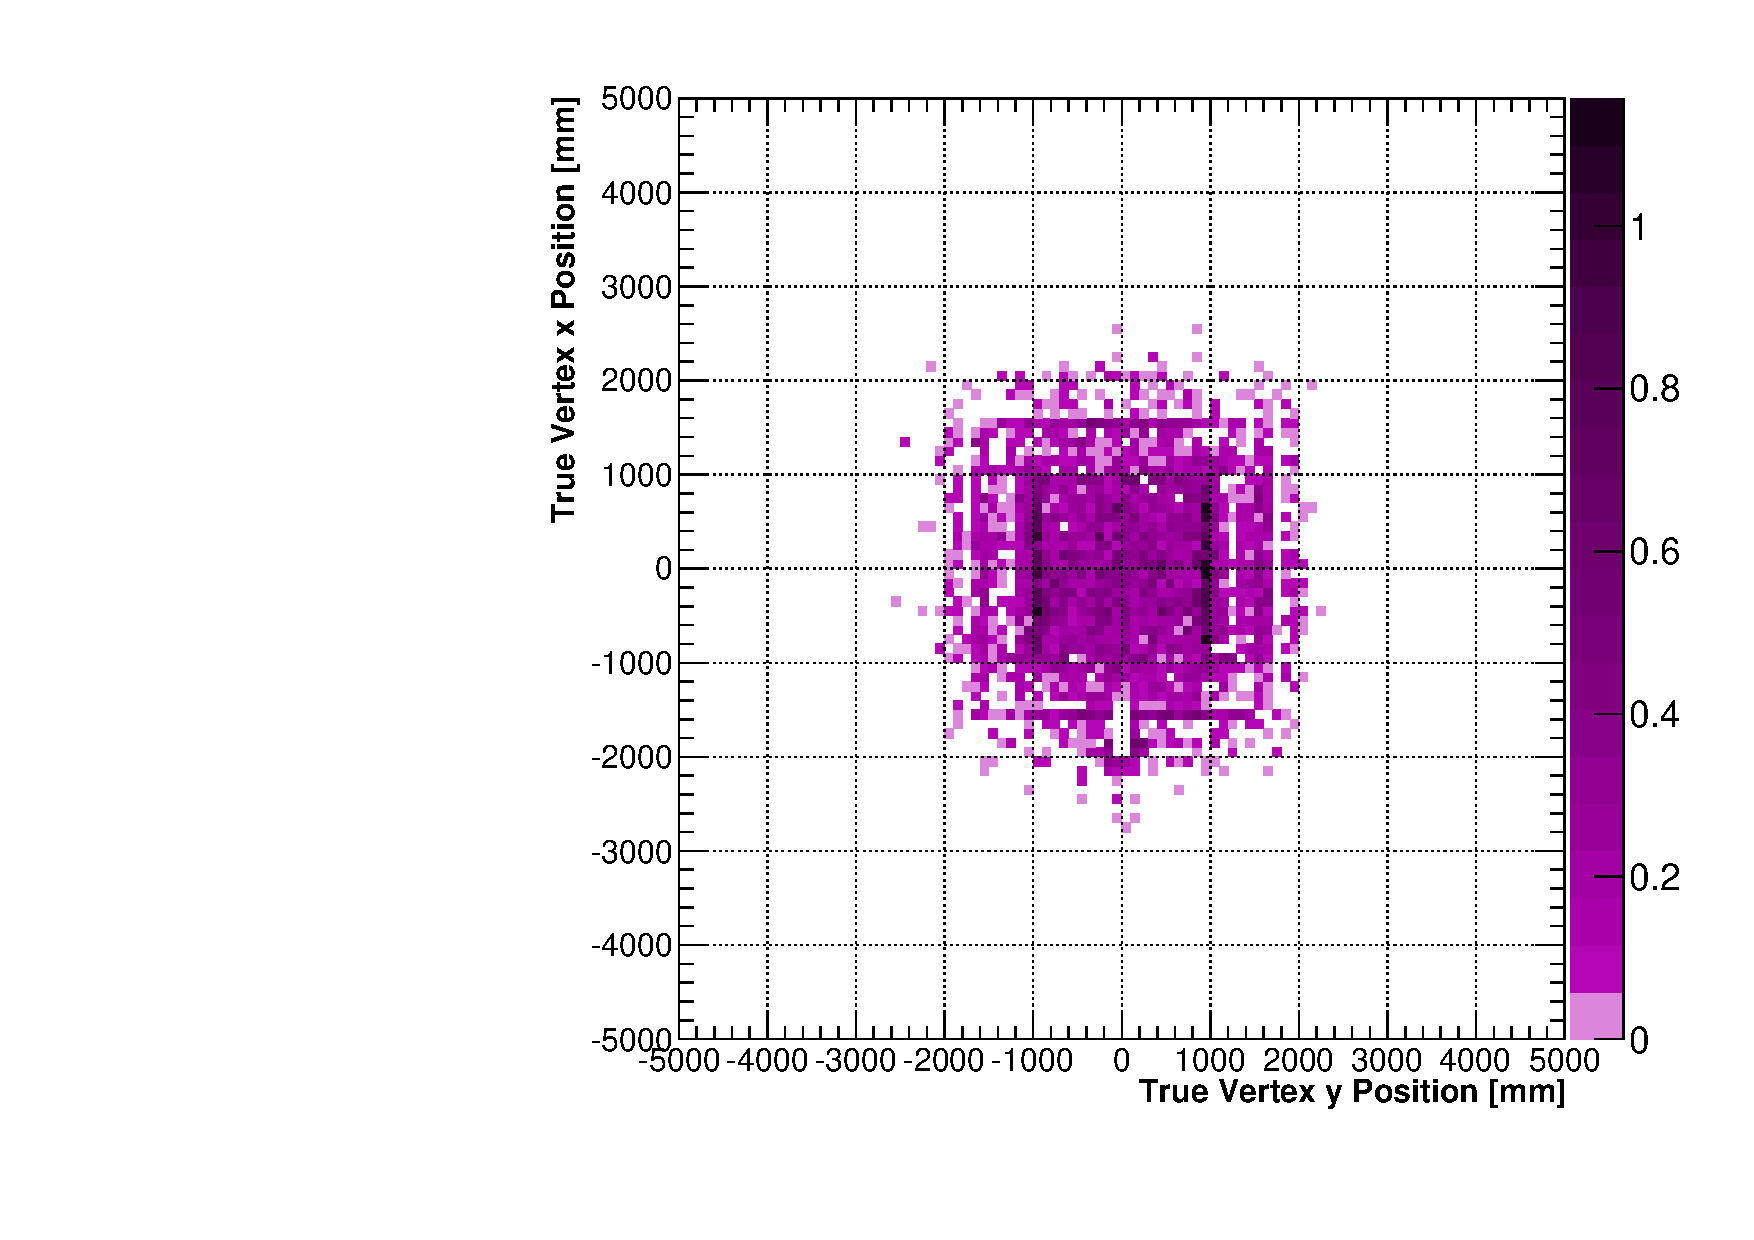
\includegraphics[width=0.48\textwidth]{images/AppOOFV/4_7.pdf}
  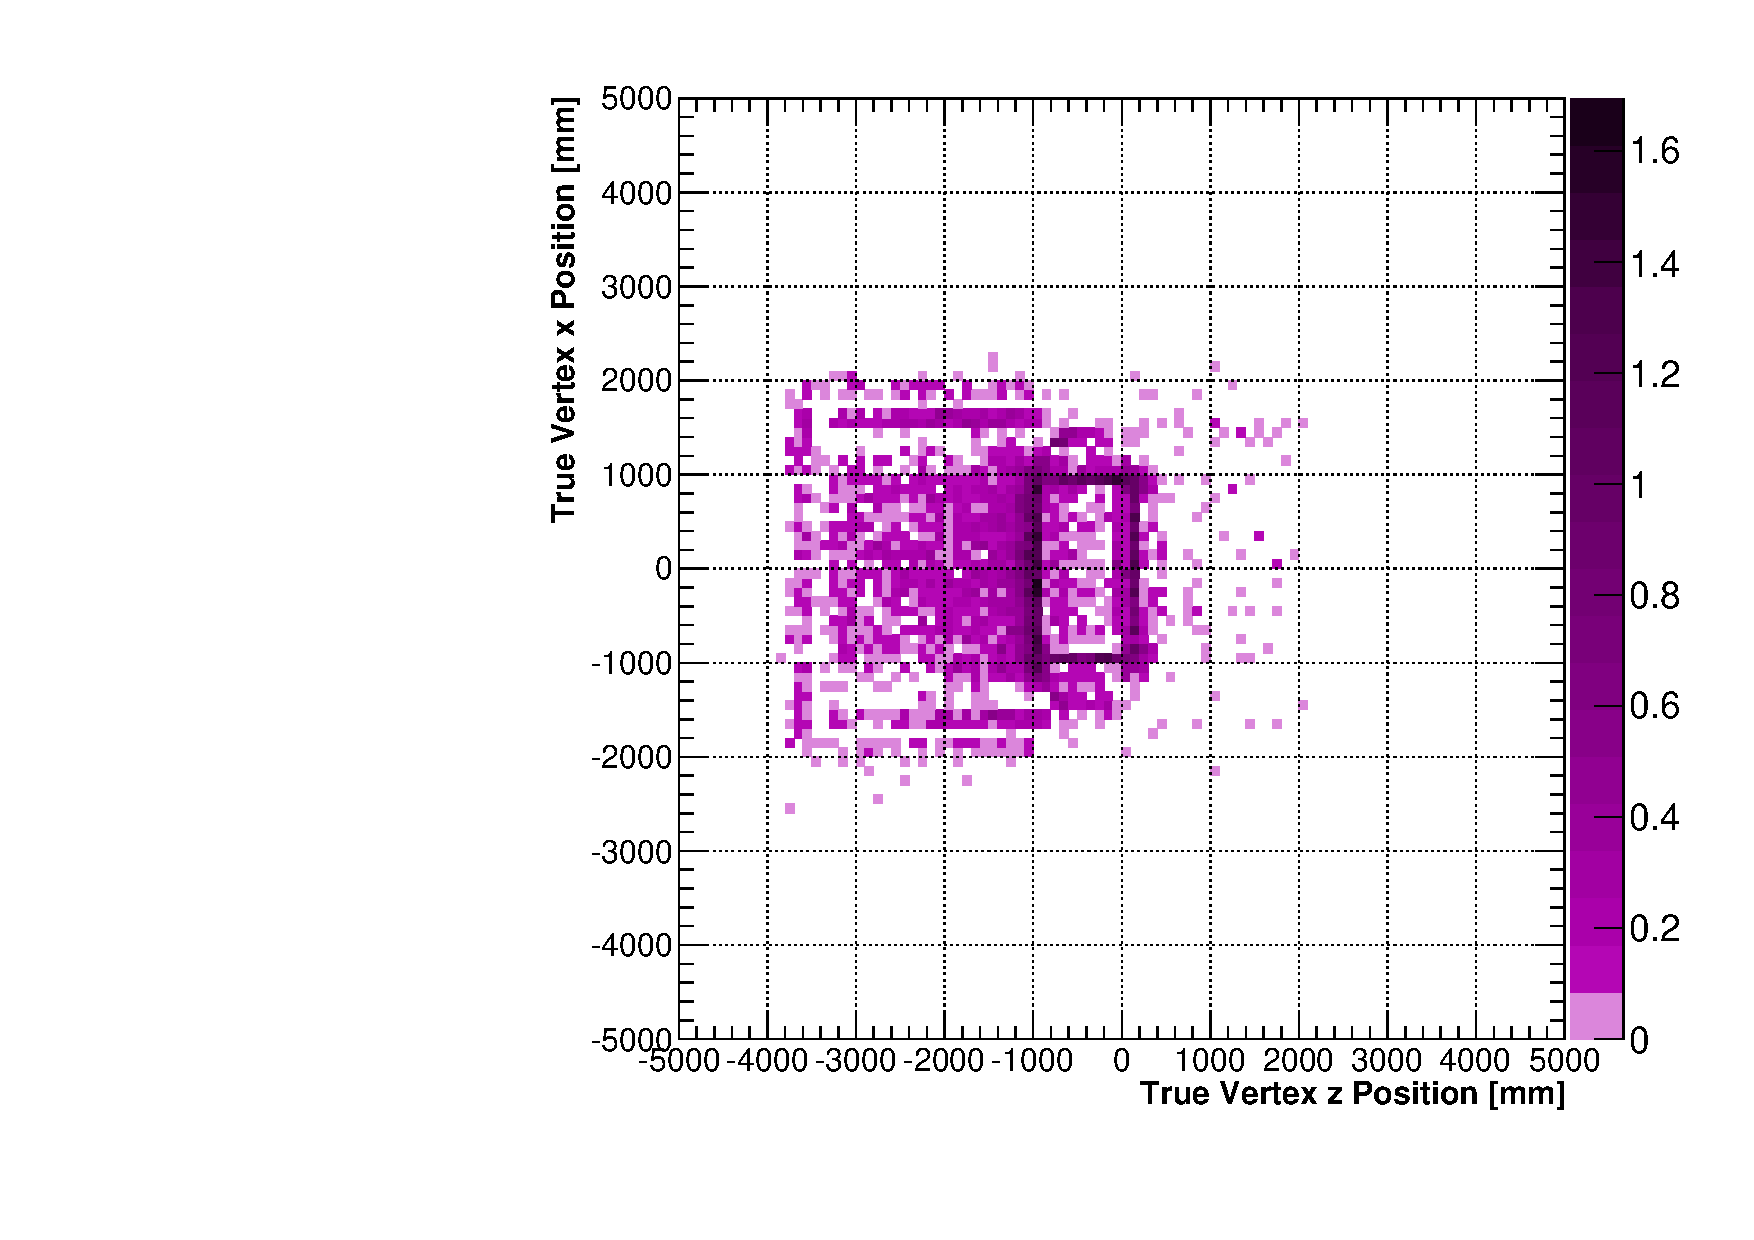
\includegraphics[width=0.48\textwidth]{images/AppOOFV/5_7.pdf}
  \caption[True positions of the OOFV events before the vetoes]{True
    positions of the true \Gls{OOFV} events before the vetoes (after
    the invariant mass cut).  \textbf{\textit{Left:}} $XY$
    projection. \textbf{\textit{Right:}} $XZ$ projection.}
  \label{fig:truepositionnovetoes}
\end{figure}

\begin{figure}[ht]
  \center
  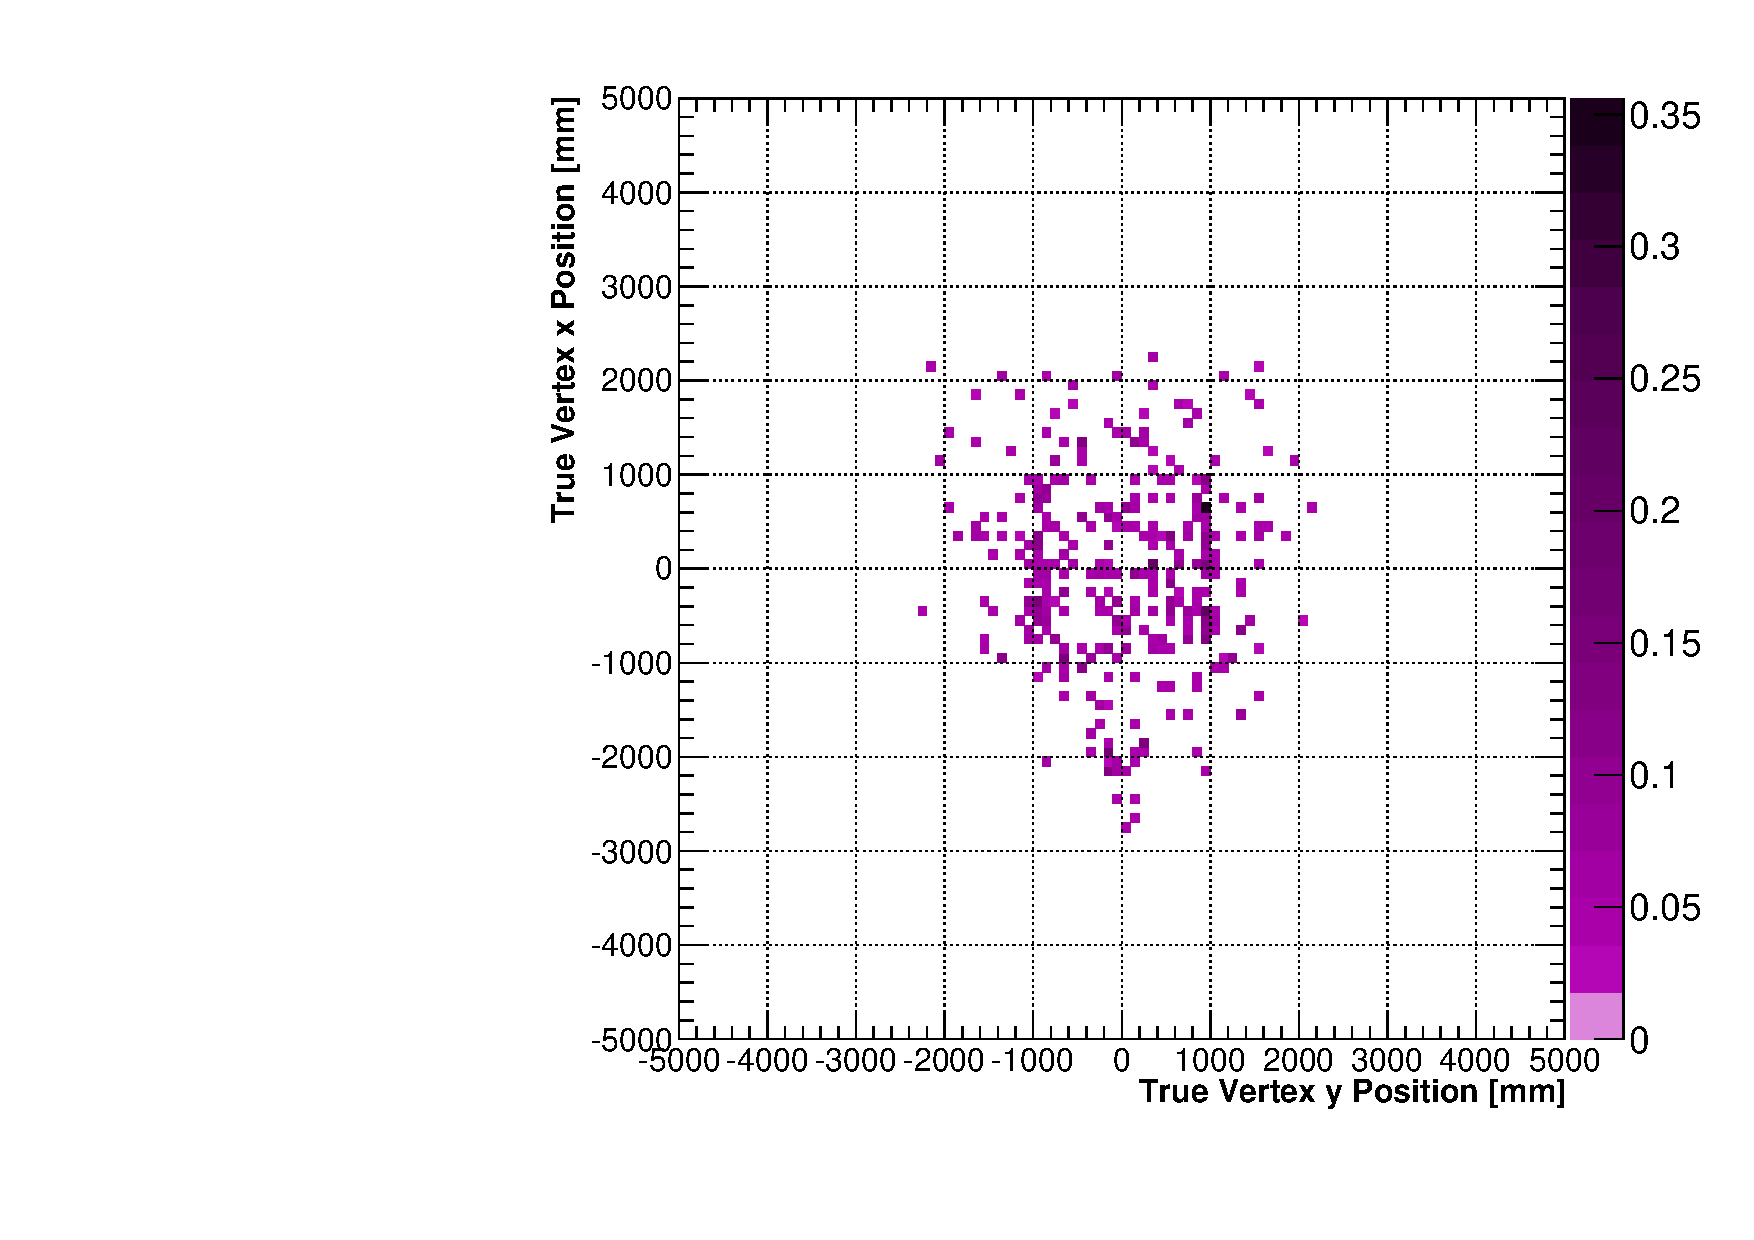
\includegraphics[width=0.48\textwidth]{images/AppOOFV/2_11.pdf}
  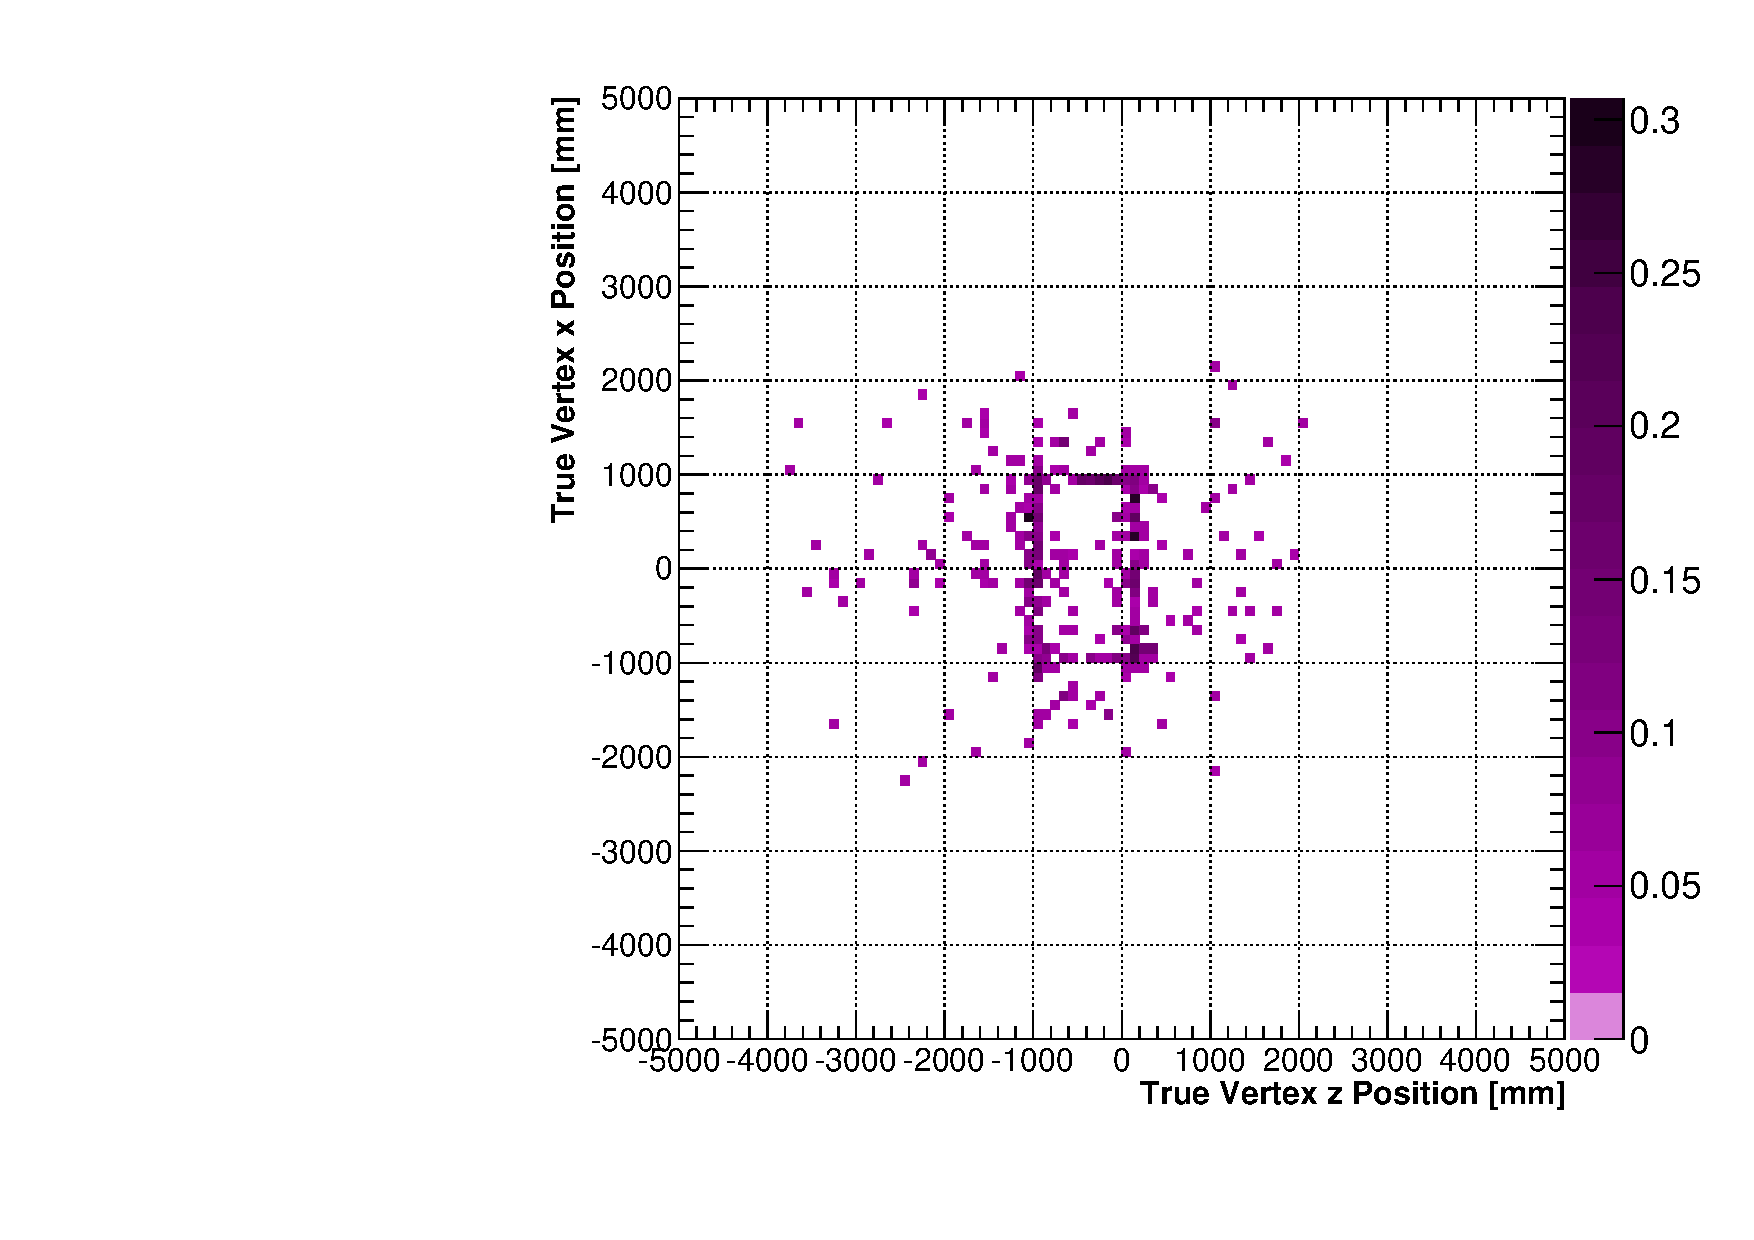
\includegraphics[width=0.48\textwidth]{images/AppOOFV/3_11.pdf}
  \caption[True positions of the OOFV events after the vetoes]{True
    positions of the true \Gls{OOFV} events after the vetoes
    (\Gls{ECal} veto). \textbf{\textit{Left:}} $XY$
    projection. \textbf{\textit{Right:}} $XZ$ projection.}
  \label{fig:truepositionwithvetoes}
\end{figure}

\begin{figure}[ht]
  \center
  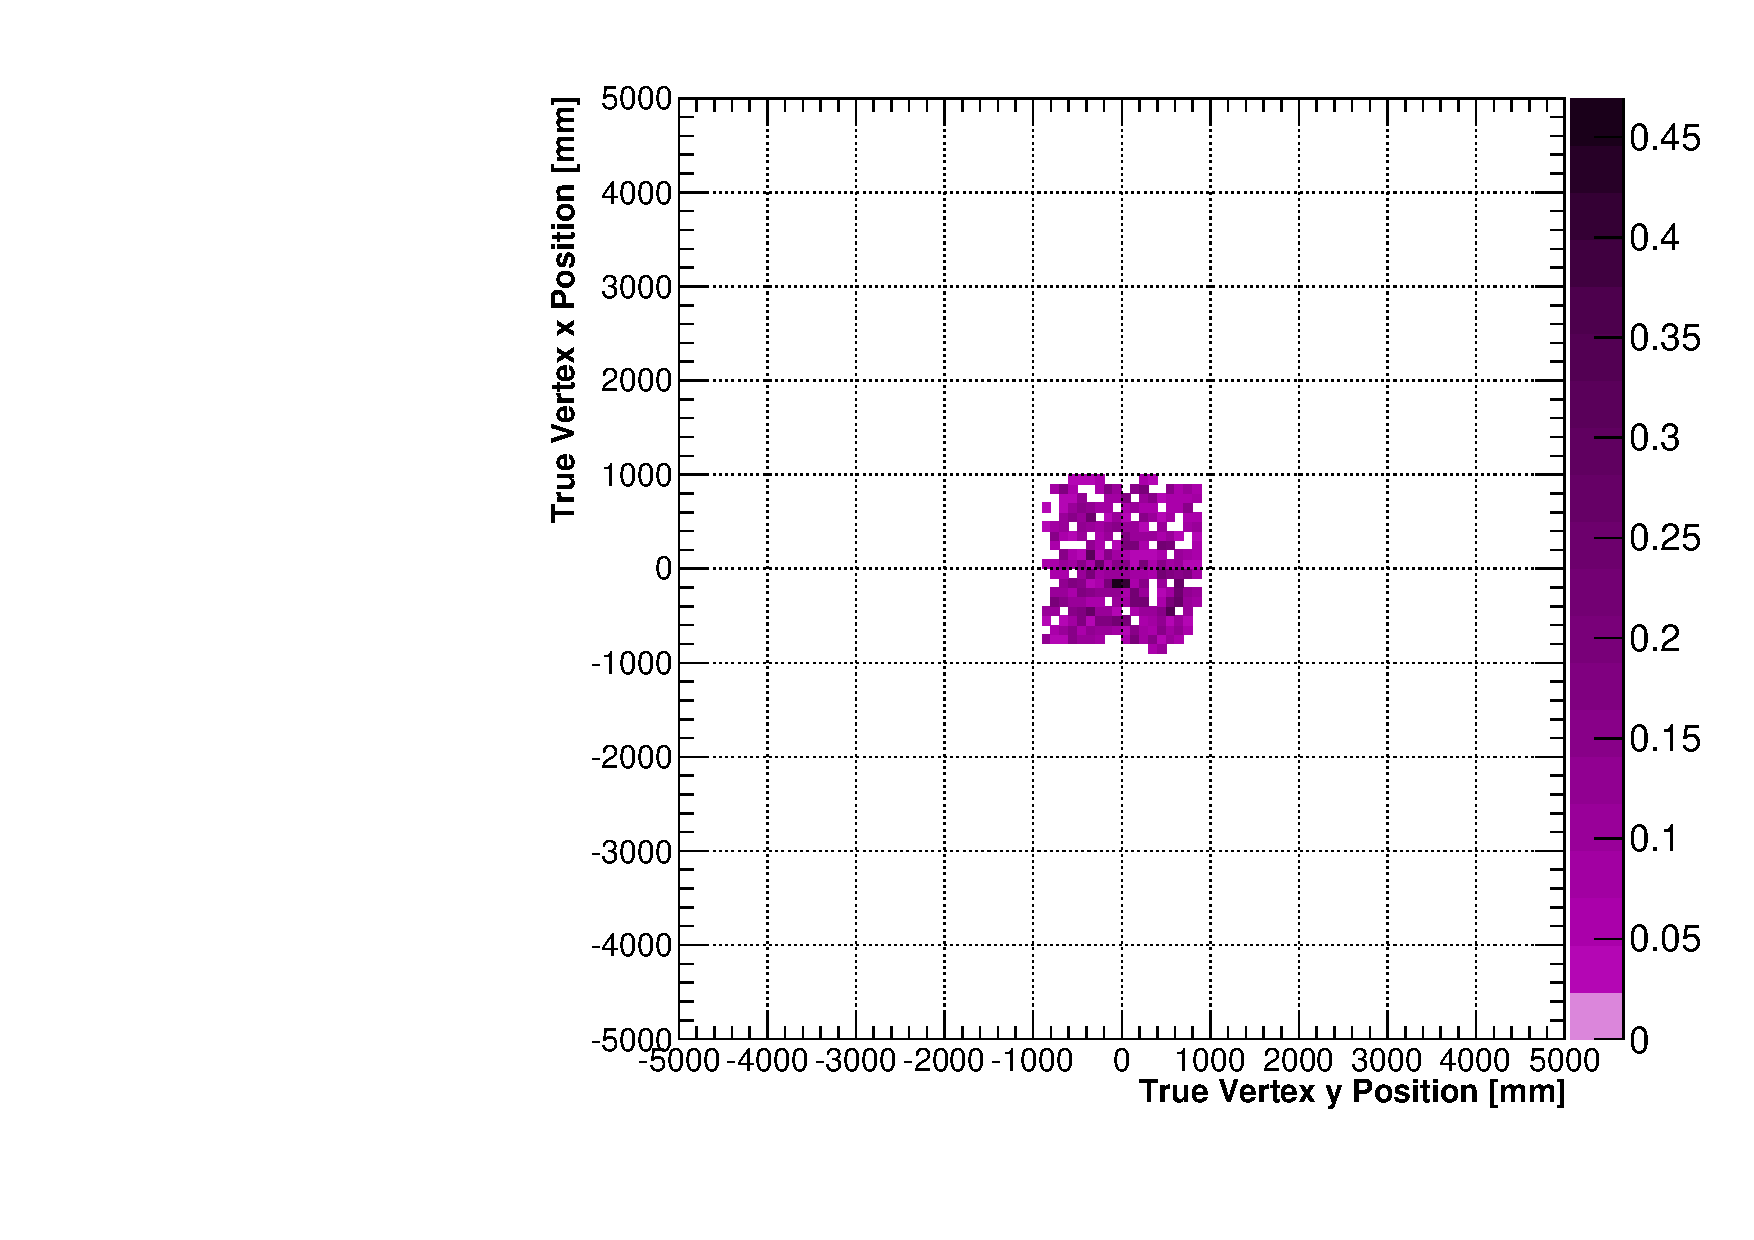
\includegraphics[width=0.48\textwidth]{images/AppOOFV/0_11.pdf}
  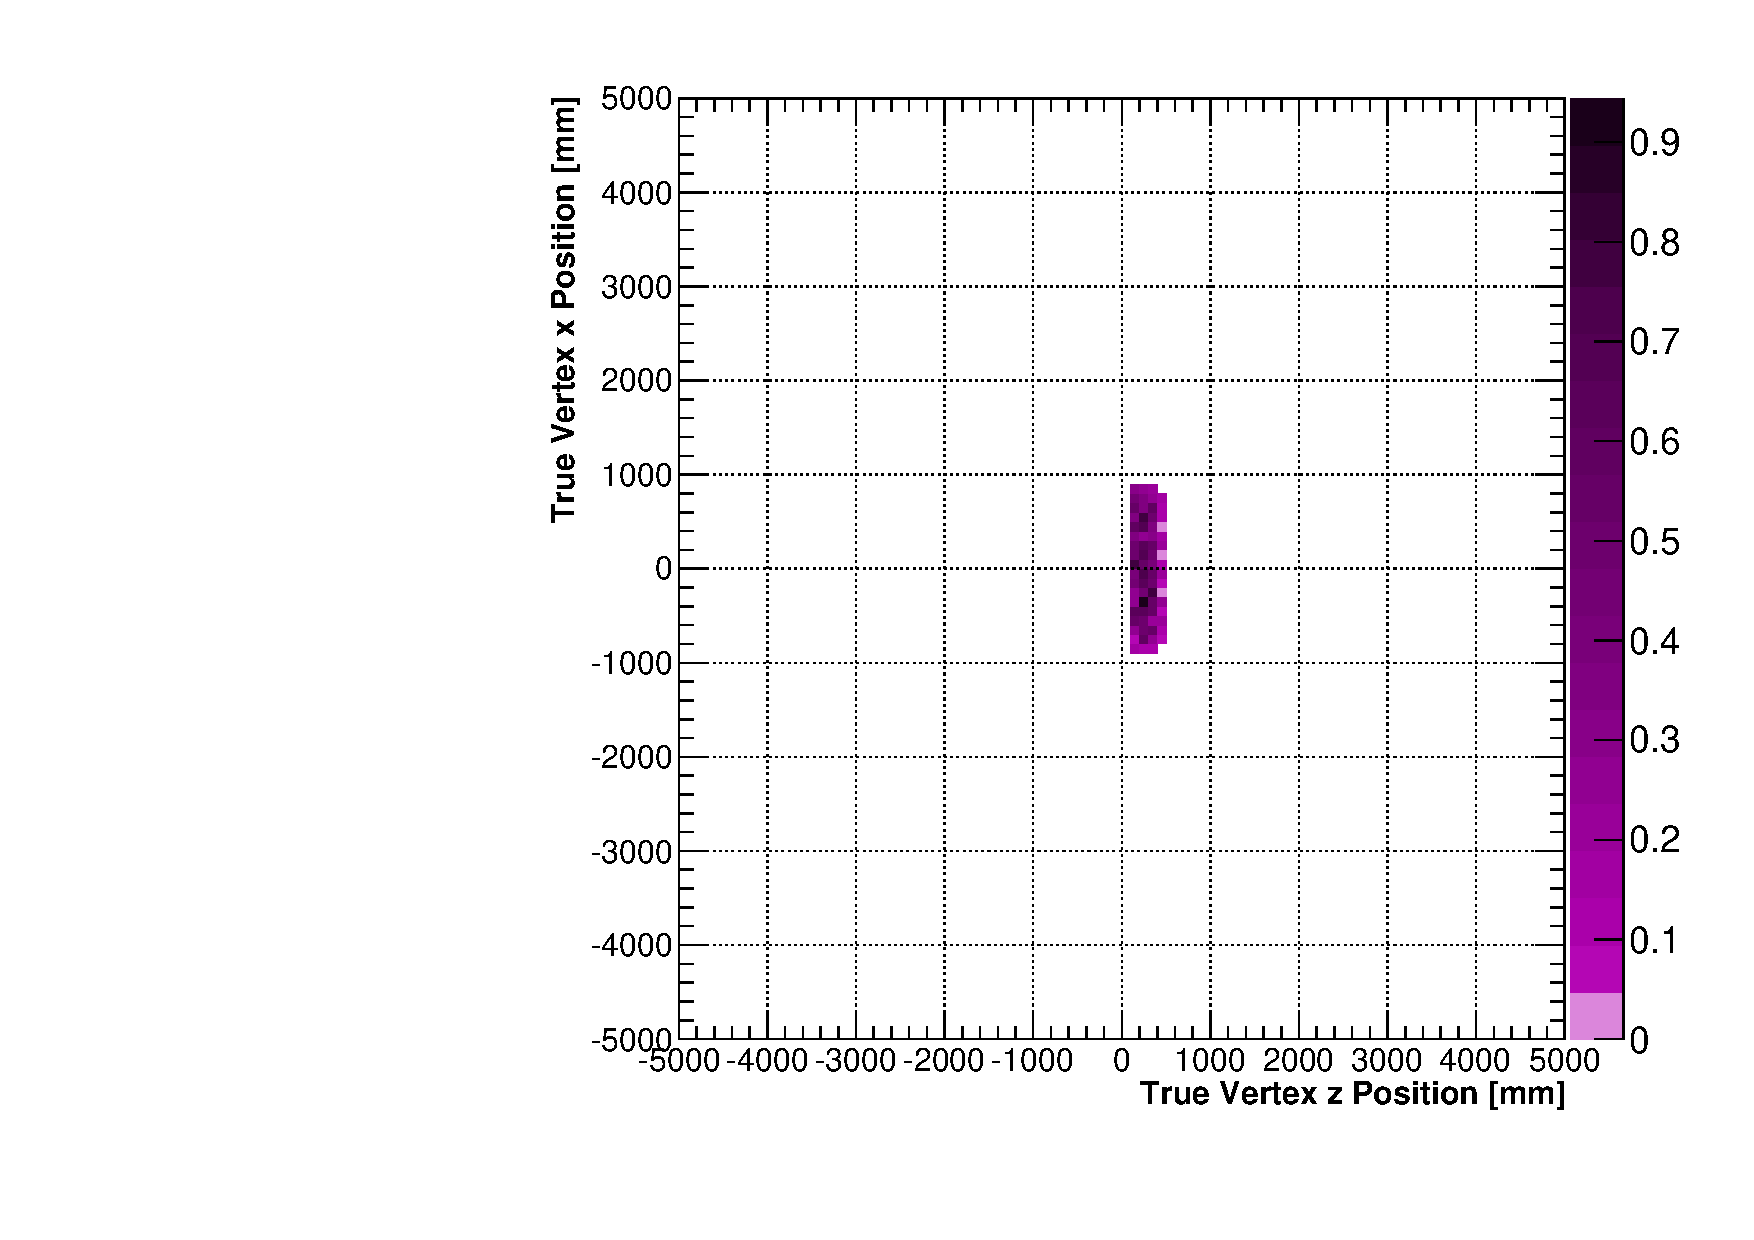
\includegraphics[width=0.48\textwidth]{images/AppOOFV/1_11.pdf}
  \caption[True positions of the FGD1 FV events after the vetoes]{True
    positions of the true \Gls{FGD}1 \Gls{FV} events after the vetoes
    (\Gls{ECal} veto). \textbf{\textit{Left:}} $XY$
    projection. \textbf{\textit{Right:}} $XZ$ projection.}
  \label{fig:truepositioninfgd}
\end{figure}




\chapter{Systematic error on the mass of the detectors}
\label{app:mass}
In this appendix, the errors on the mass of each detector is
detailed. The \Gls{PD}, \Gls{ECal} and \Gls{FGD} mass uncertainties
are reported, as well as the errors for those events which originates
from the other regions of the \Gls{ND}, that are not the \Glspl{FGD},
\Gls{ECal} and \Gls{PD}. These regions are later called Out Of All
Fiducial Volumes (\Gls{OOAFV}).

All these errors are used in Section~\ref{subsec:photonsec}, where the
systematic error for the ``out of fiducial volume'' photons is
explained.

\section*{The \Gls{FGD} mass uncertainty}
The \Gls{FGD} mass uncertainty is known and is
$0.6\%$, see Section~\ref{subsec:fgdmass}.

\section*{The \Gls{PD} mass uncertainty}
\label{par:podmassuncertainty}
For the \Gls{PD} mass uncertainty, the error is directly extracted
from~\cite{TN258}, where the corrections are summed to the errors
reported for simplicity. This leads to the mass uncertainties listed
on Table~\ref{tab:podmass}. To get the numbers corresponding to the
mass proportions for the two configurations (with and without water),
the masses of the components reported in~\cite{P0Dpaper2012} were
used.

\begin{table}[ht]
  \center
  \begin{tabular}{cccc}
    \toprule
    Component & Mass uncertainty    & Proportion with water & Proportion without water \\ 
    \midrule
    Water     & 2.16~\%      & 22.25~\% & 0~\% \\
    Brass     & 17.8~\%      & 8.54~\%  & 10.98~\% \\
    Lead      & 2.3~\%       & 21.84~\% & 28.08~\% \\
    Other     & 0.95~\%      & 47.37~\% & 60.93~\% \\
    \bottomrule
  \end{tabular}
  \caption[P0D components mass uncertainties]{\Gls{PD} components mass
    uncertainties.}
  \label{tab:podmass}
\end{table}

\section*{The \Gls{ECal} mass uncertainty}
\label{par:ecalmassuncertainty}
The errors for the masses of the \Gls{ECal} componenent were retrieved
from~\cite{DomBrailsford2016}, however, rather than computing the
covariance matrix between the different components of the \Gls{ECal},
the uncertainties in the dimensions of the different components of the
\Gls{ECal} were simply added in quadrature. The uncertainties in the
sizes of the holes for the fibre in the scintillators were neglected
since they are very small compared to the overall size of the
bars. Similarly, the masses of the fibres were neglected. In
Table~\ref{tab:ecalmass}, the uncertainties and proportions of the
various components are shown for the \Gls{BrECal} modules (note that
the \Gls{DsECal} is irrelevant for this study, since no photon come
from the \Gls{DsECal} in the analysis). The relatively large mass
uncertainties comes from the fact that the errors on the widths of the
scintillator bars are quite large (this also applies for the lead
layers).

\begin{table}[ht]
  \center
  \tabcolsep=0.11cm
  \begin{tabular}{llcccc}
    \toprule
    Bar type    & Size and error [$mm$]                                        & \#/layer & $\rho [g/cm^3]$& $\delta$~mass    & Proportion \\ 
    \midrule
    \multicolumn{6}{l}{Top~/~bottom modules} \\
    \midrule
    Scintillator & $(3840 \pm 0.1) \times (40  \pm 0.4) \times (10   \pm 0.4)$  & 38           & 1                 & 4.12~\%             & 24.96~\%   \\
    Scintillator & $(1520 \pm 0.1) \times (40  \pm 0.4) \times (10   \pm 0.4)$  & 96           & 1                 & 4.12~\%             & 24.96~\%   \\
    Lead         & $(3858 \pm 4)   \times (765 \pm 4)   \times (1.75 \pm 0.1)$  & 2            & 11.34             & 5.74~\%             & 50.08~\%   \\
    Total        &                                                              &              &                   & 4.93~\%             & 100~\%     \\
    \midrule
    \multicolumn{6}{l}{Left~/~right modules} \\
    \midrule
    Scintillator & $(3840  \pm 0.1) \times (40   \pm 0.4) \times (10   \pm 0.4)$  & 57           & 1                 & 4.12~\%             & 24.77~\%   \\
    Scintillator & $(2280  \pm 0.1) \times (40   \pm 0.4) \times (10   \pm 0.4)$  & 96           & 1                 & 4.12~\%             & 24.77~\%   \\
    Lead         & $(964.5 \pm 4)   \times (2330 \pm 4)   \times (1.75 \pm 0.1)$  & 4            & 11.34             & 5.73~\%             & 50.46~\%   \\
    Total        &                                                                &              &                   & 4.93~\%             & 100~\%     \\
    \bottomrule
  \end{tabular}
  \caption[BrECal bars masses and uncertainties]{\Gls{BrECal} bars
    masses and uncertainties.}
  \label{tab:ecalmass}
\end{table}

\section*{The \Gls{OOAFV} mass uncertainties}
\label{par:oofvmassuncertainty}
Each detector in the \Gls{ND} has a mass uncertainty, however it is
not trivial to estimate the errors on the masses of the dead materials
in the \Gls{ND}. For that, a control sample was constructed with the
aim of uncovering possible errors in mass modelling at the \Gls{ND}.

A \Gls{CC} inclusive selection was performed on the edges of the
\Gls{FGD}1. The selection is briefly described below:

\begin{itemize}[noitemsep,topsep=0pt]
\item The track is required to have more than 18 nodes in the
  \Gls{TPC} and to start in the \Gls{FGD}1 detector (note that this
  does not necessarily have to be in its \Gls{FV}).
\item The events were vetoed when activity (one or more reconstructed
  tracks) was seen in the \Gls{BrECal}, in the \Gls{PD} and more
  importantly in the \Gls{TPC}1. The aim of these vetoes is to remove
  the \gls{sand} muons and the \Gls{ECal} interactions.
\item Next, the events were classified according to whether they would
  come from the edges of the \Gls{FGD}1 (which are the ``signal regions'')
  or inside the fiducial volume of the \Gls{FGD}1 (later used as
  side-band region).
\end{itemize}

That way, the selection is dominated by interactions occurring on the
edges of the scintillator of \Gls{FGD}1 and in the dead material
surrounding it, as illustrated in
Figures~\ref{fig:oofvcontrolsampletrue}~and~\ref{fig:oofvcontrolsamplereco}.

\begin{figure}[ht]
  \center
  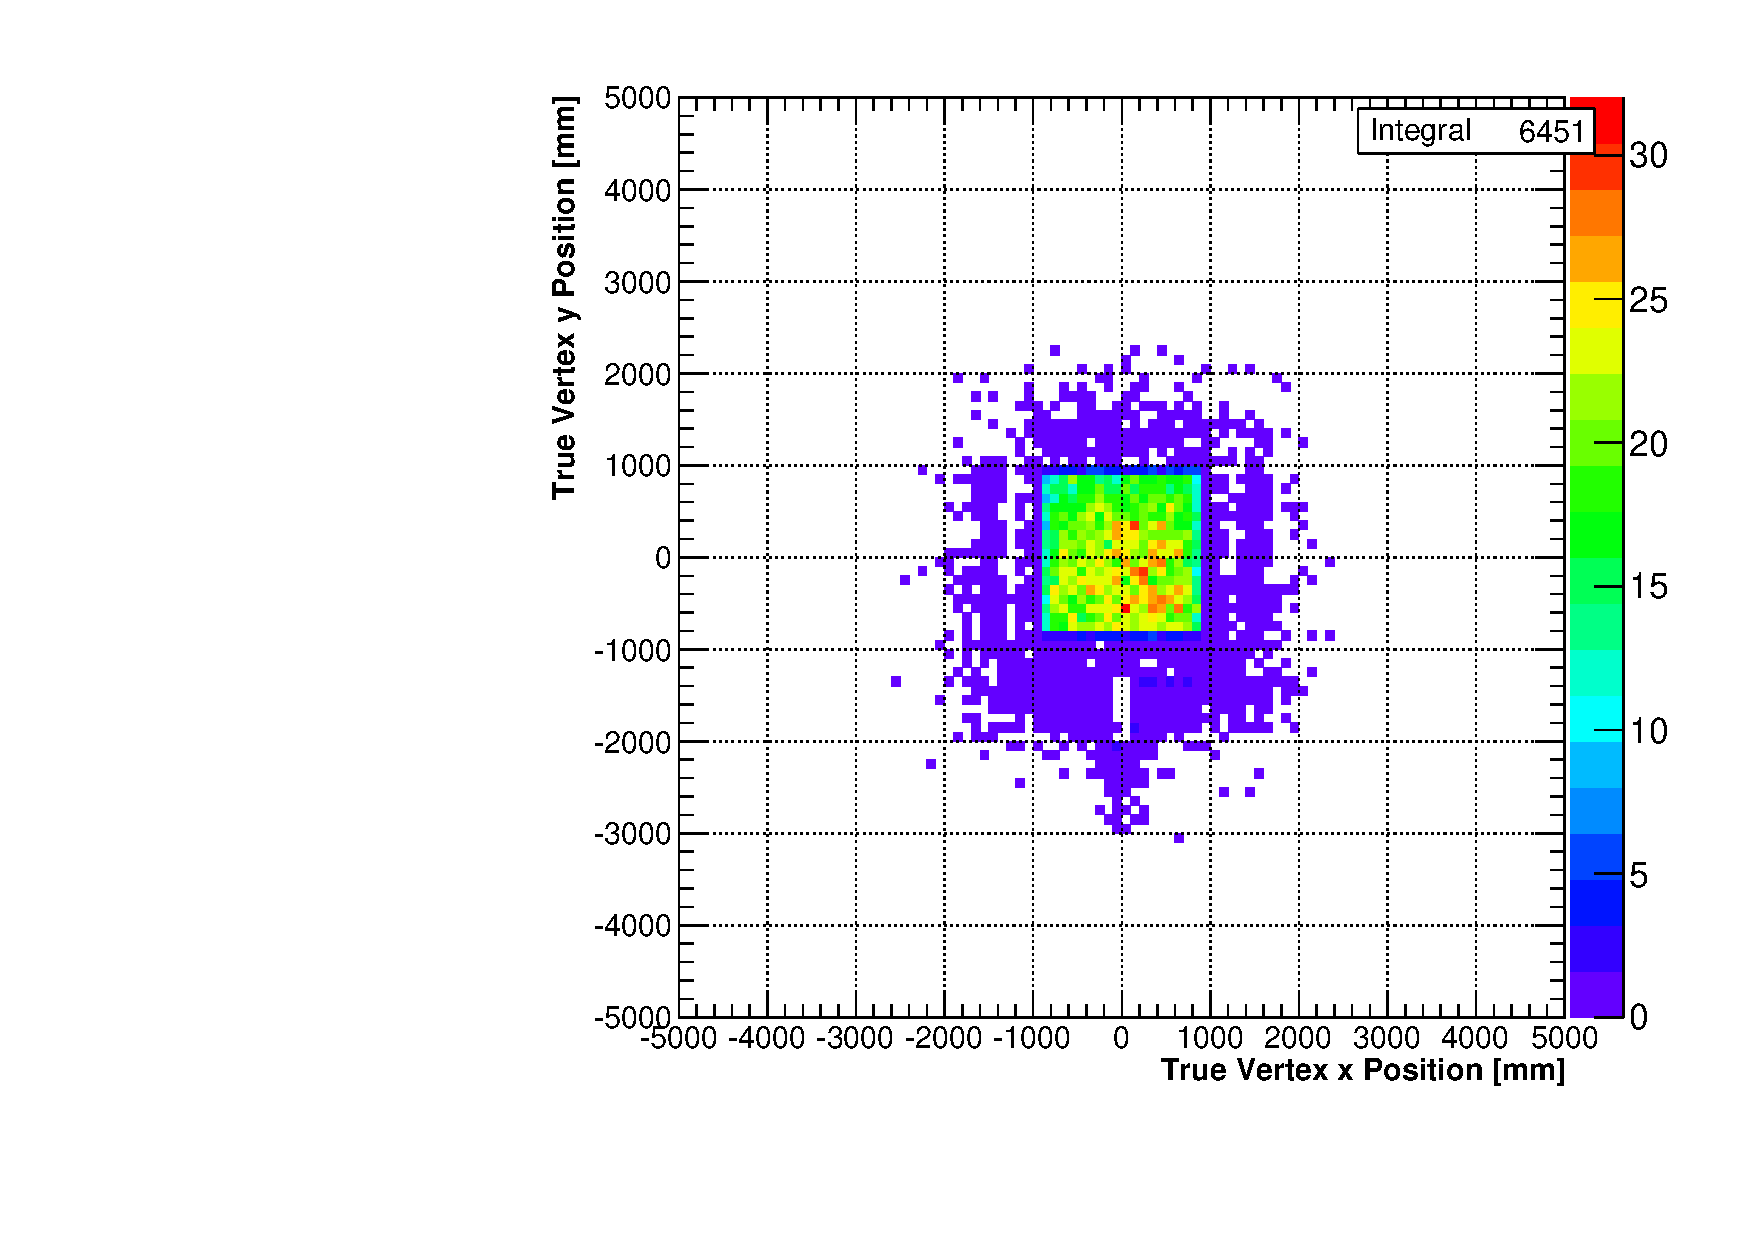
\includegraphics[width=0.48\textwidth]{T2K-TN-313/images/systematics/xy_infv_true.pdf}
  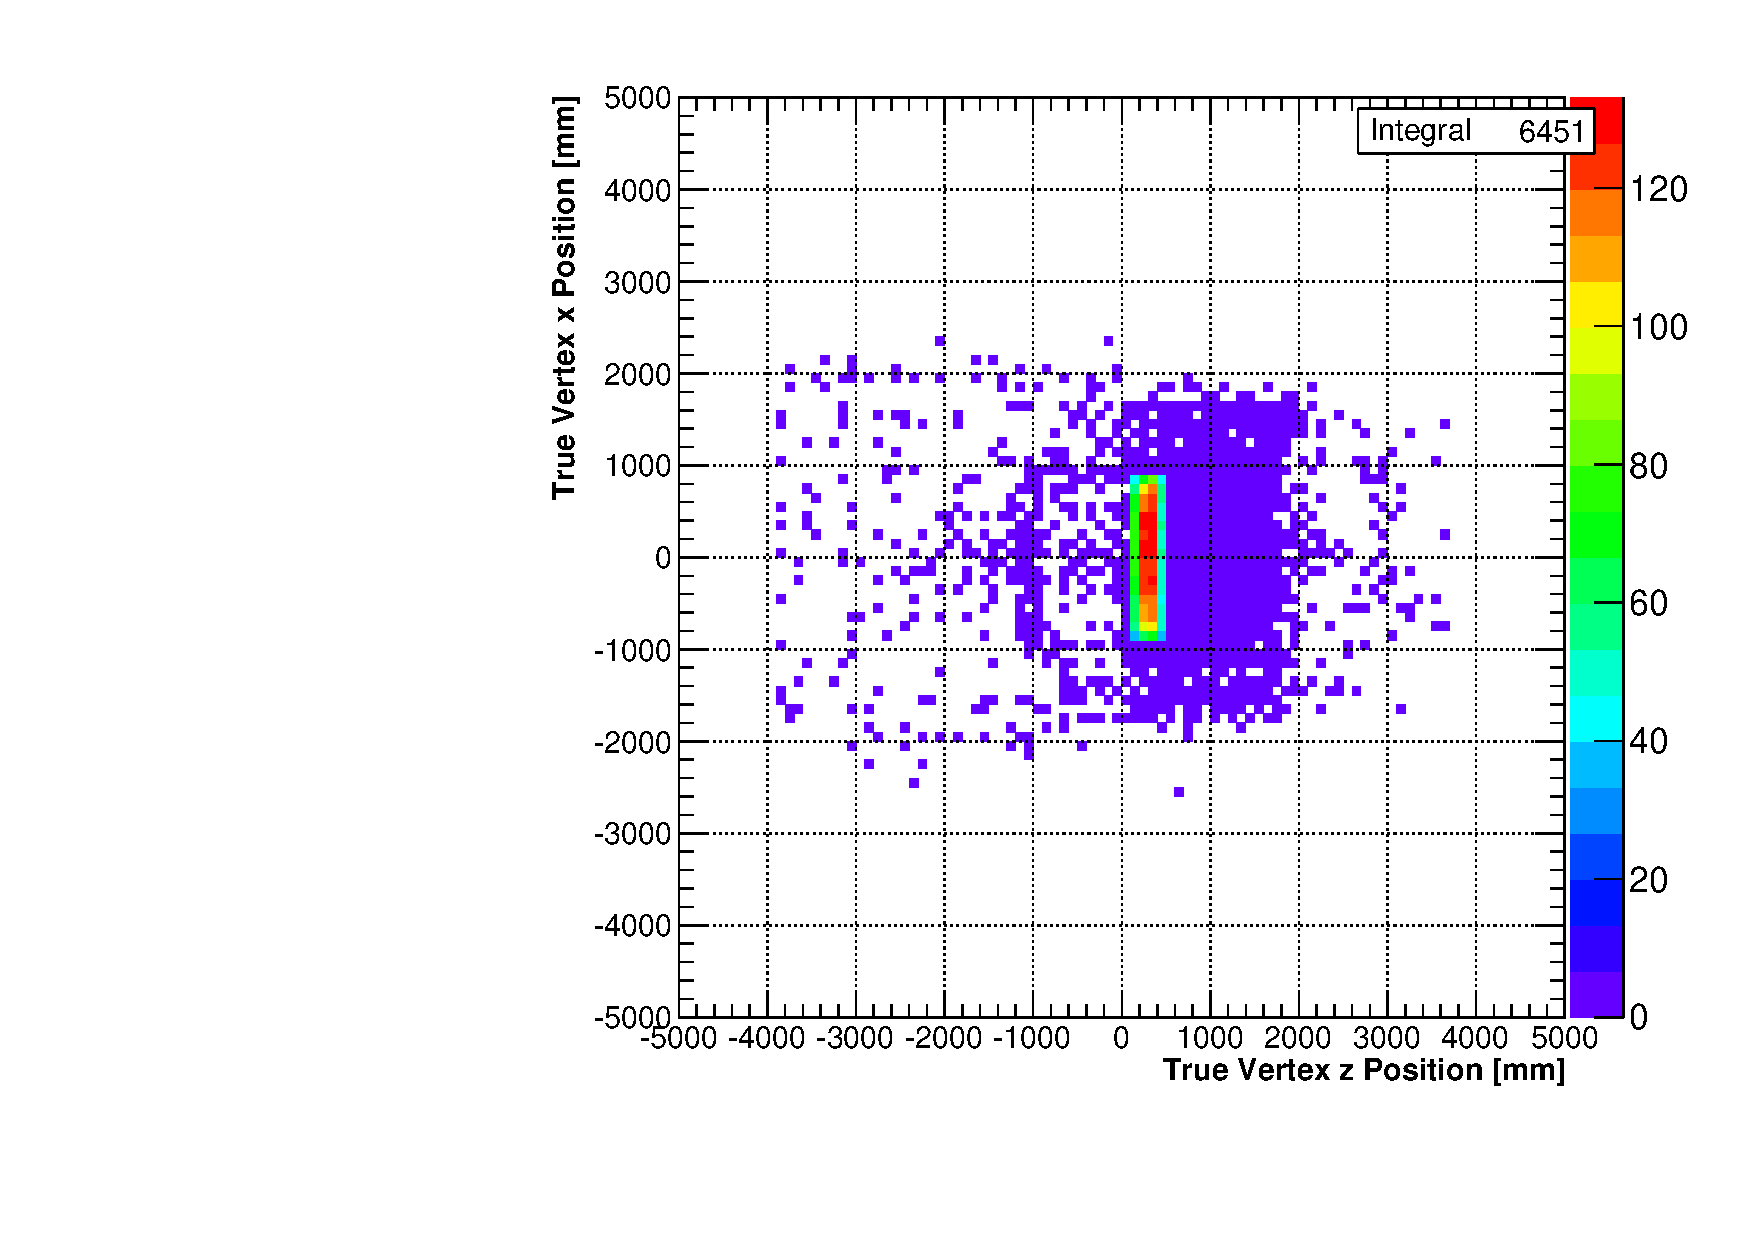
\includegraphics[width=0.48\textwidth]{T2K-TN-313/images/systematics/xz_infv_true.pdf} \\
  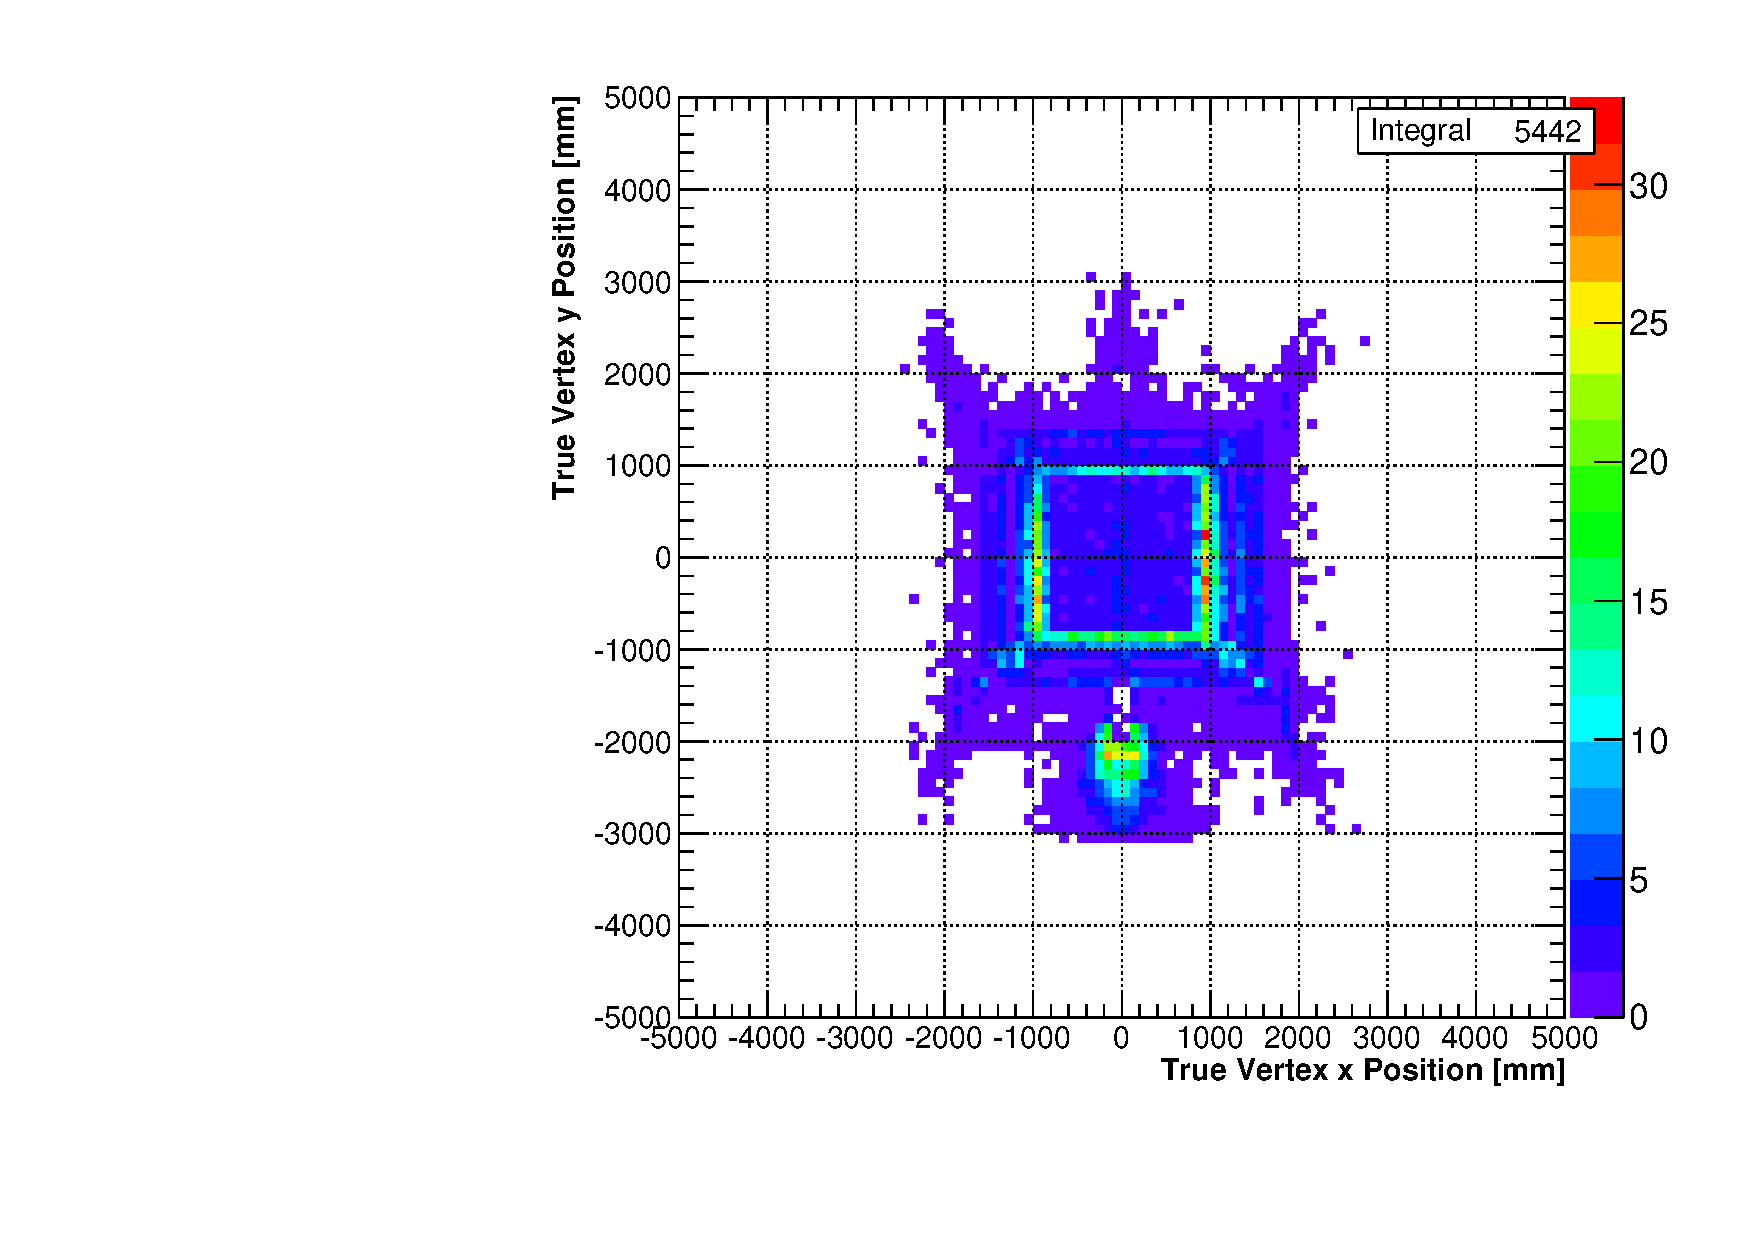
\includegraphics[width=0.48\textwidth]{T2K-TN-313/images/systematics/xy_oofv_true.pdf}
  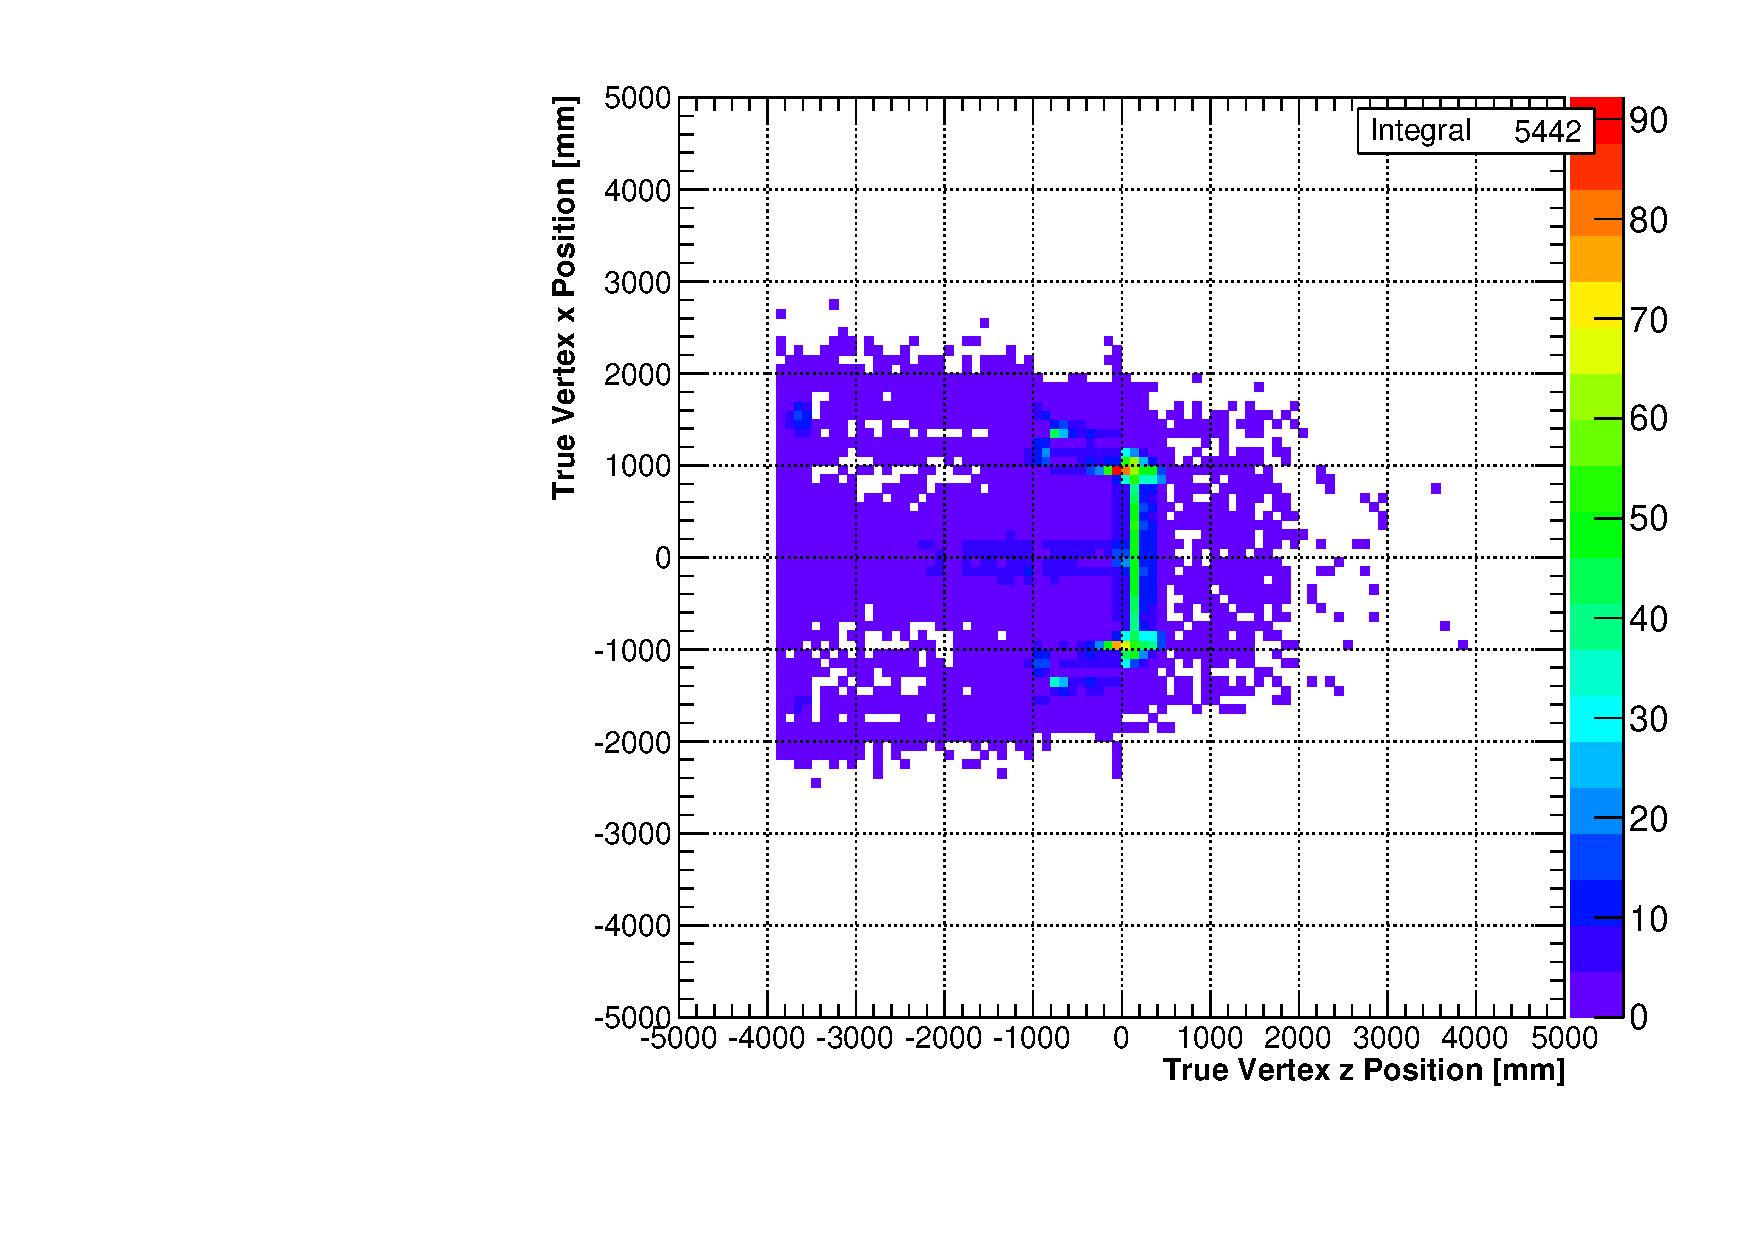
\includegraphics[width=0.48\textwidth]{T2K-TN-313/images/systematics/xz_oofv_true.pdf} \\
  \caption[True positions of the events selected for the estimation of the OOAFV error]{True
    positions of vertices for the events selected for the estimation of the \Gls{OOAFV} error.
    \textbf{\textit{Top left:}} Inside the \Gls{FGD}1 \Gls{FV}, $XY$ plane projection.
    \textbf{\textit{Top right:}} Inside the \Gls{FGD}1 \Gls{FV}, $XZ$ plane projection.
    \textbf{\textit{Bottom left:}} Outside the \Gls{FGD}1 \Gls{FV}, $XY$ plane projection.
    \textbf{\textit{Bottom right:}} Outside the \Gls{FGD}1 \Gls{FV}, $XZ$ plane projection.
  }
  \label{fig:oofvcontrolsampletrue}
\end{figure}

\begin{figure}[ht]
  \center
  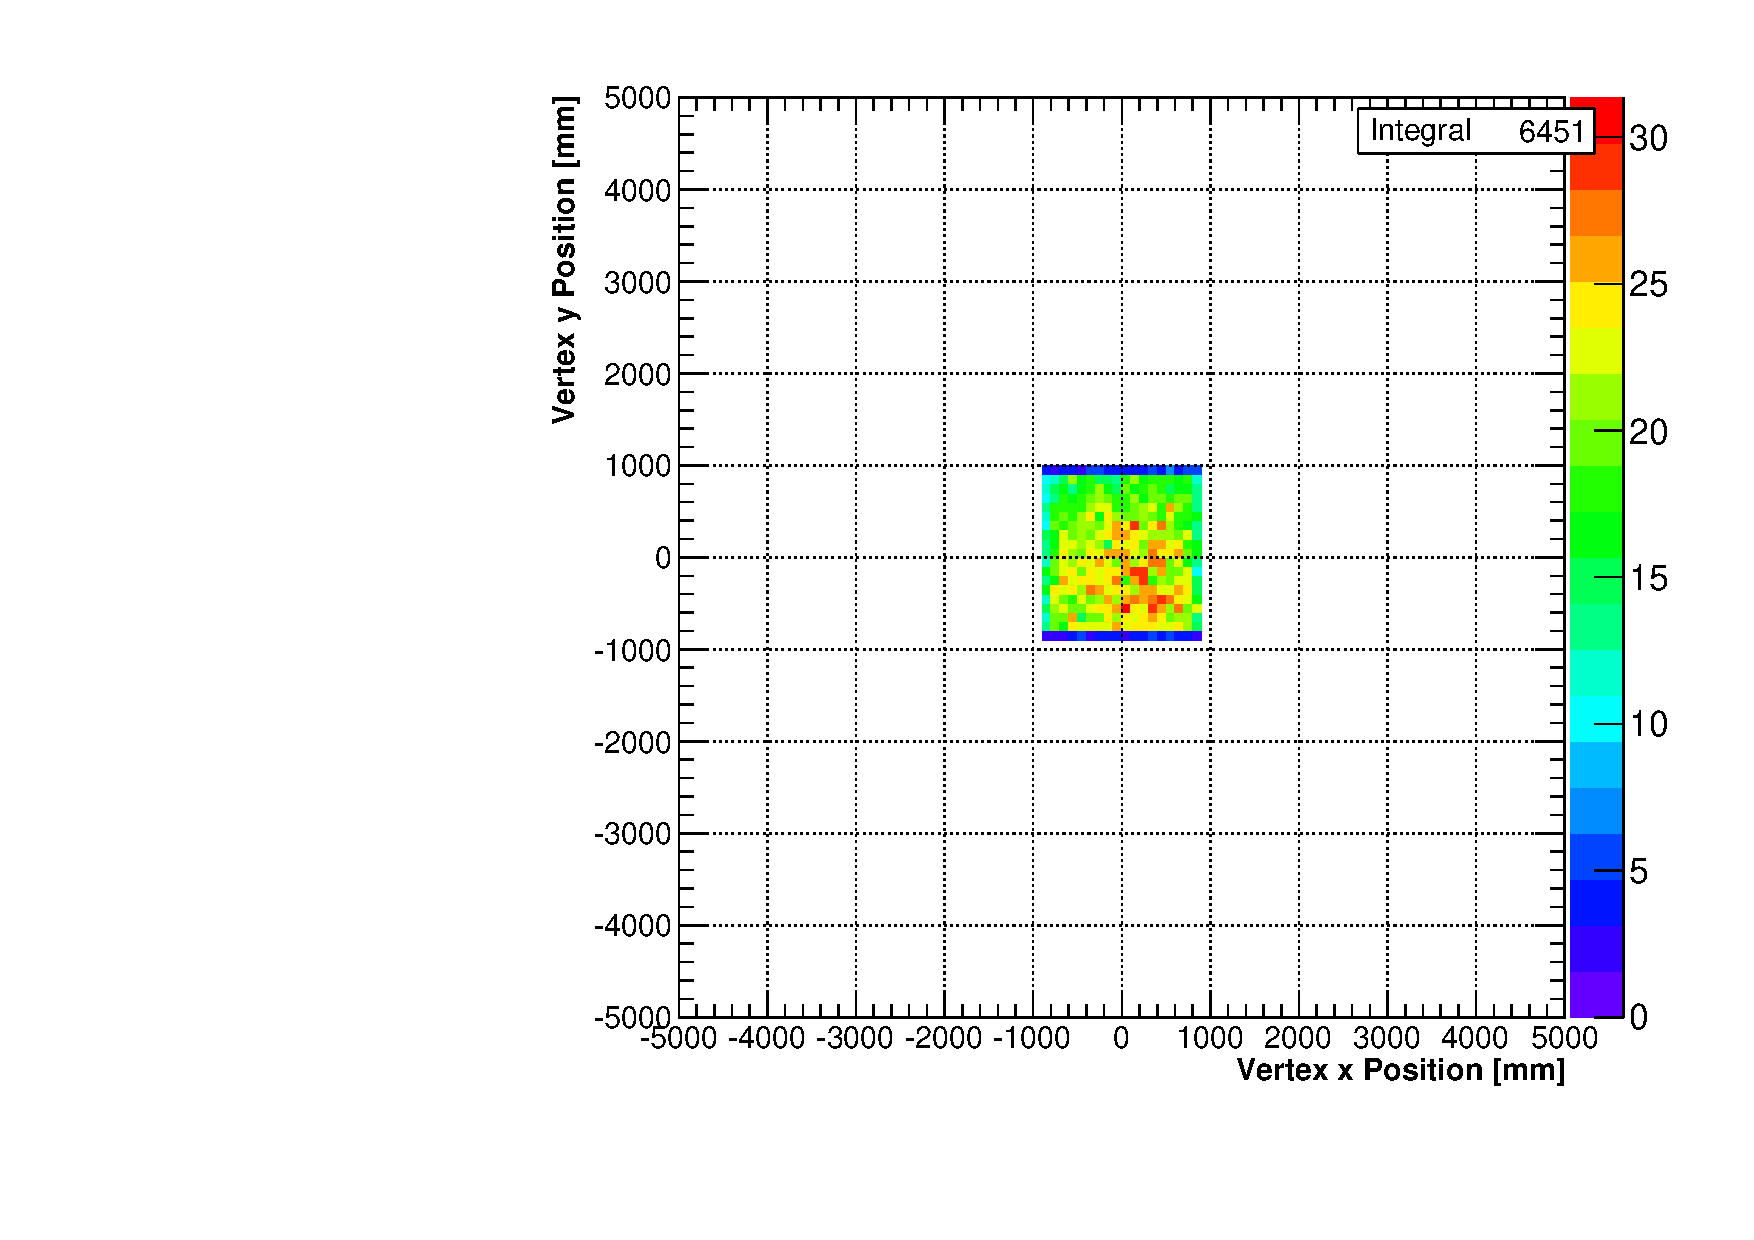
\includegraphics[width=0.48\textwidth]{T2K-TN-313/images/systematics/xy_infv_reco.pdf}
  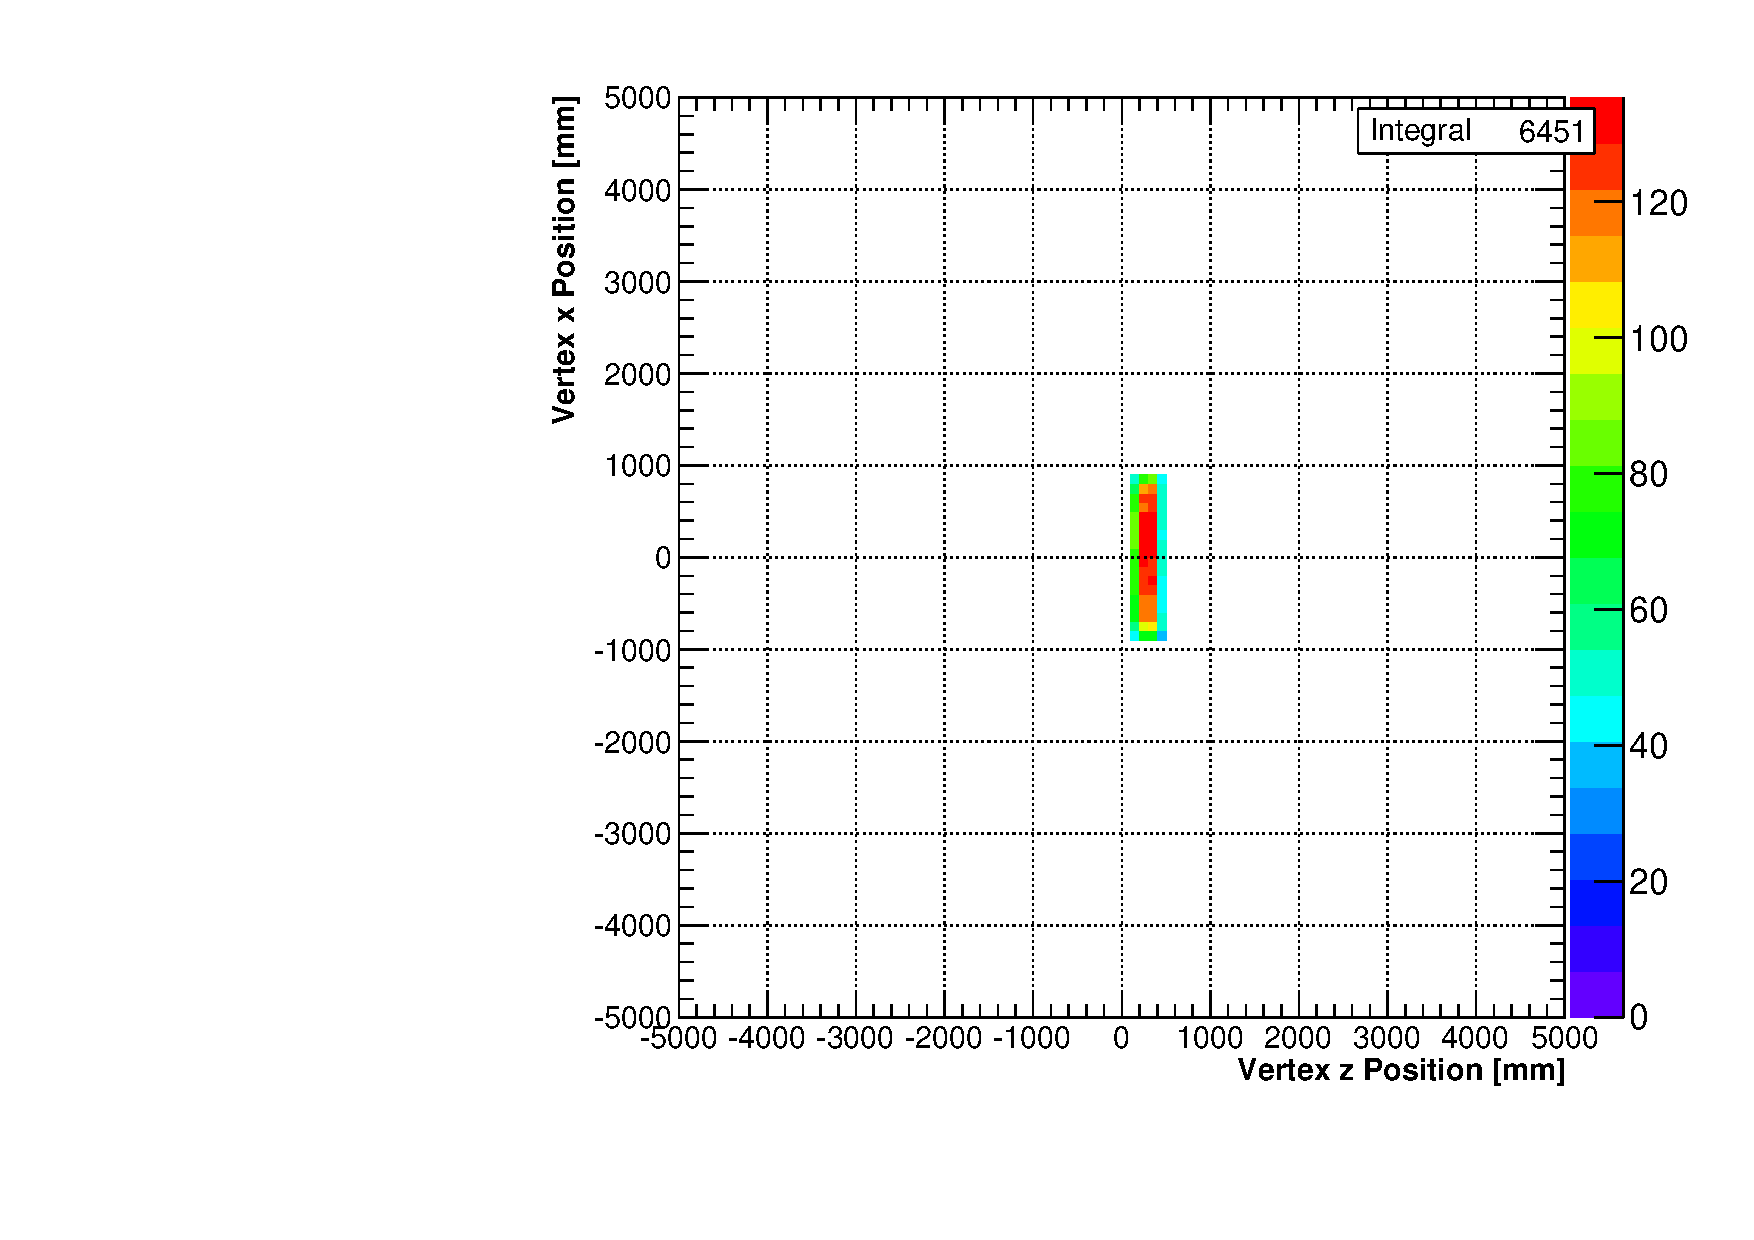
\includegraphics[width=0.48\textwidth]{T2K-TN-313/images/systematics/xz_infv_reco.pdf} \\
  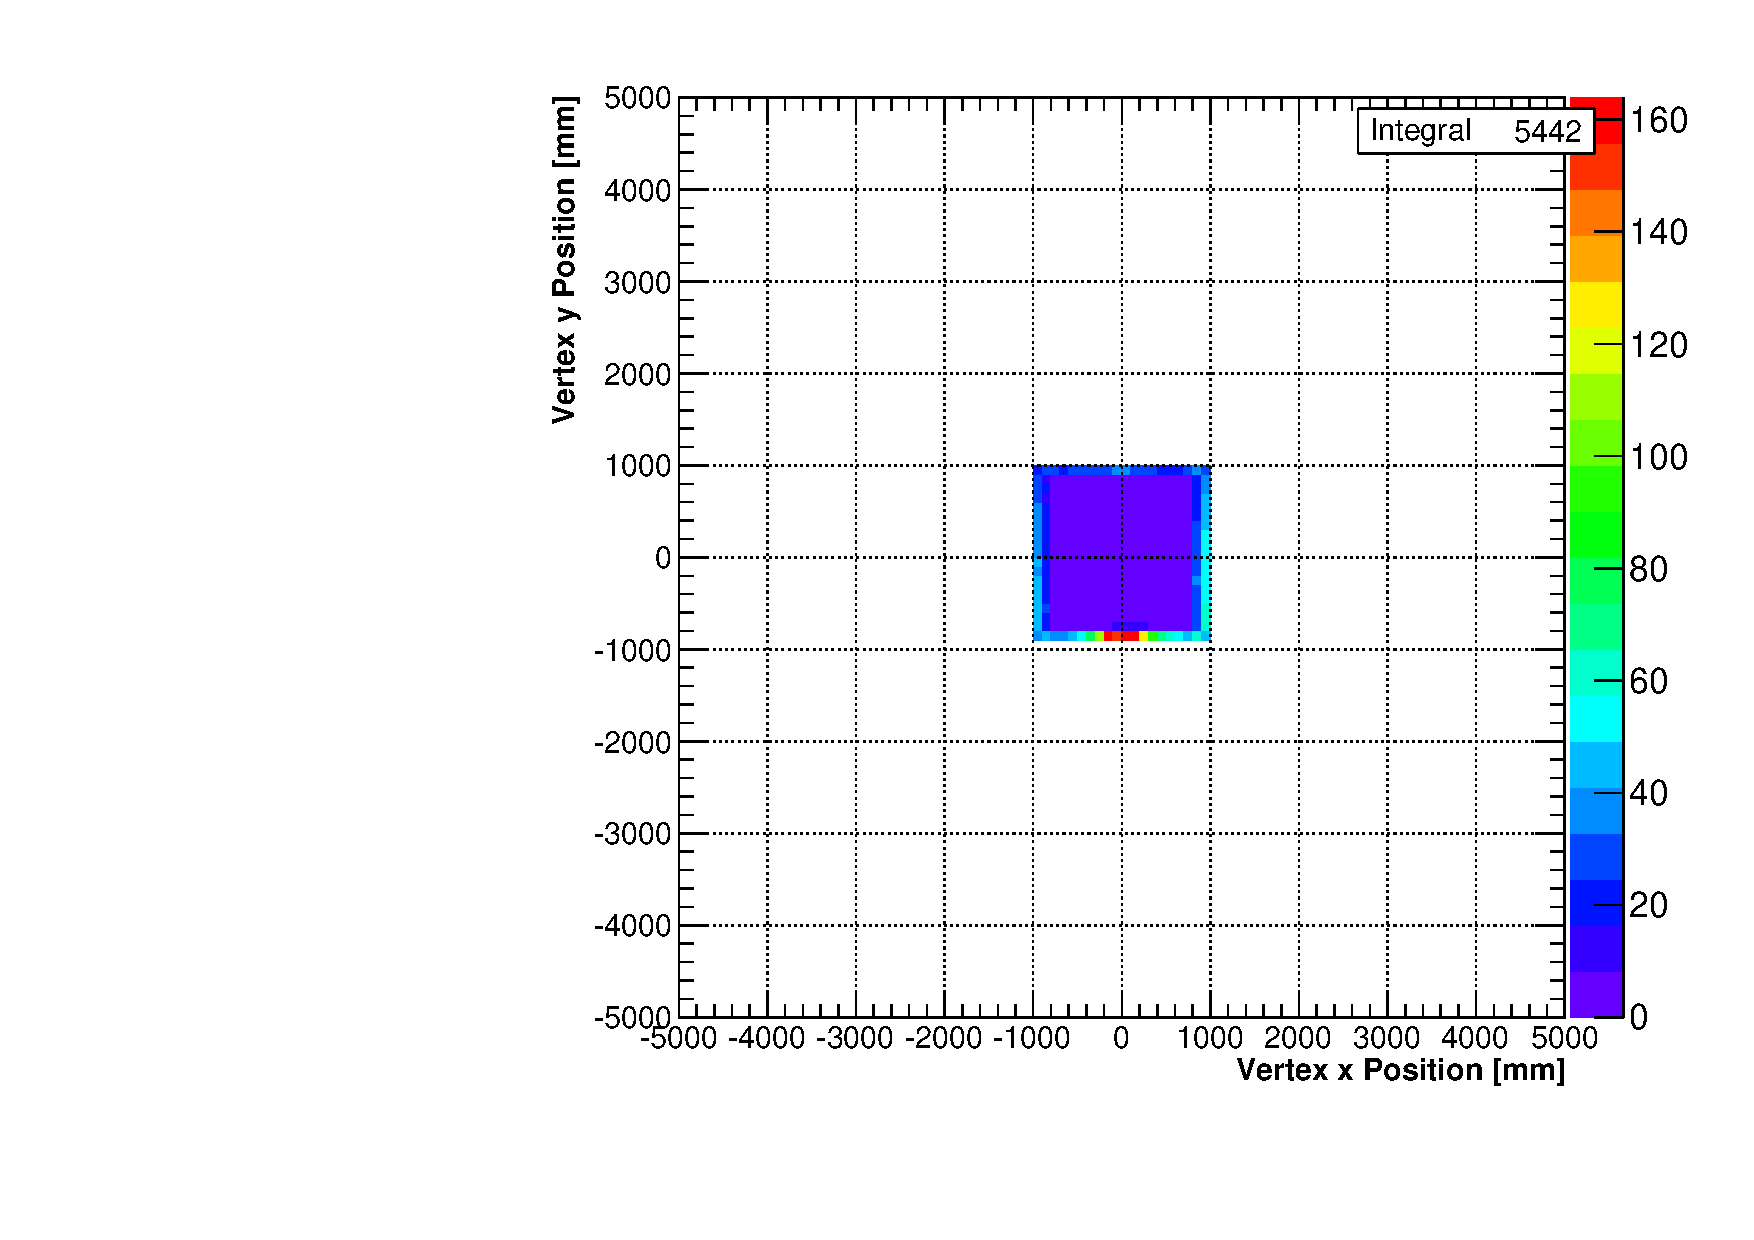
\includegraphics[width=0.48\textwidth]{T2K-TN-313/images/systematics/xy_oofv_reco.pdf}
  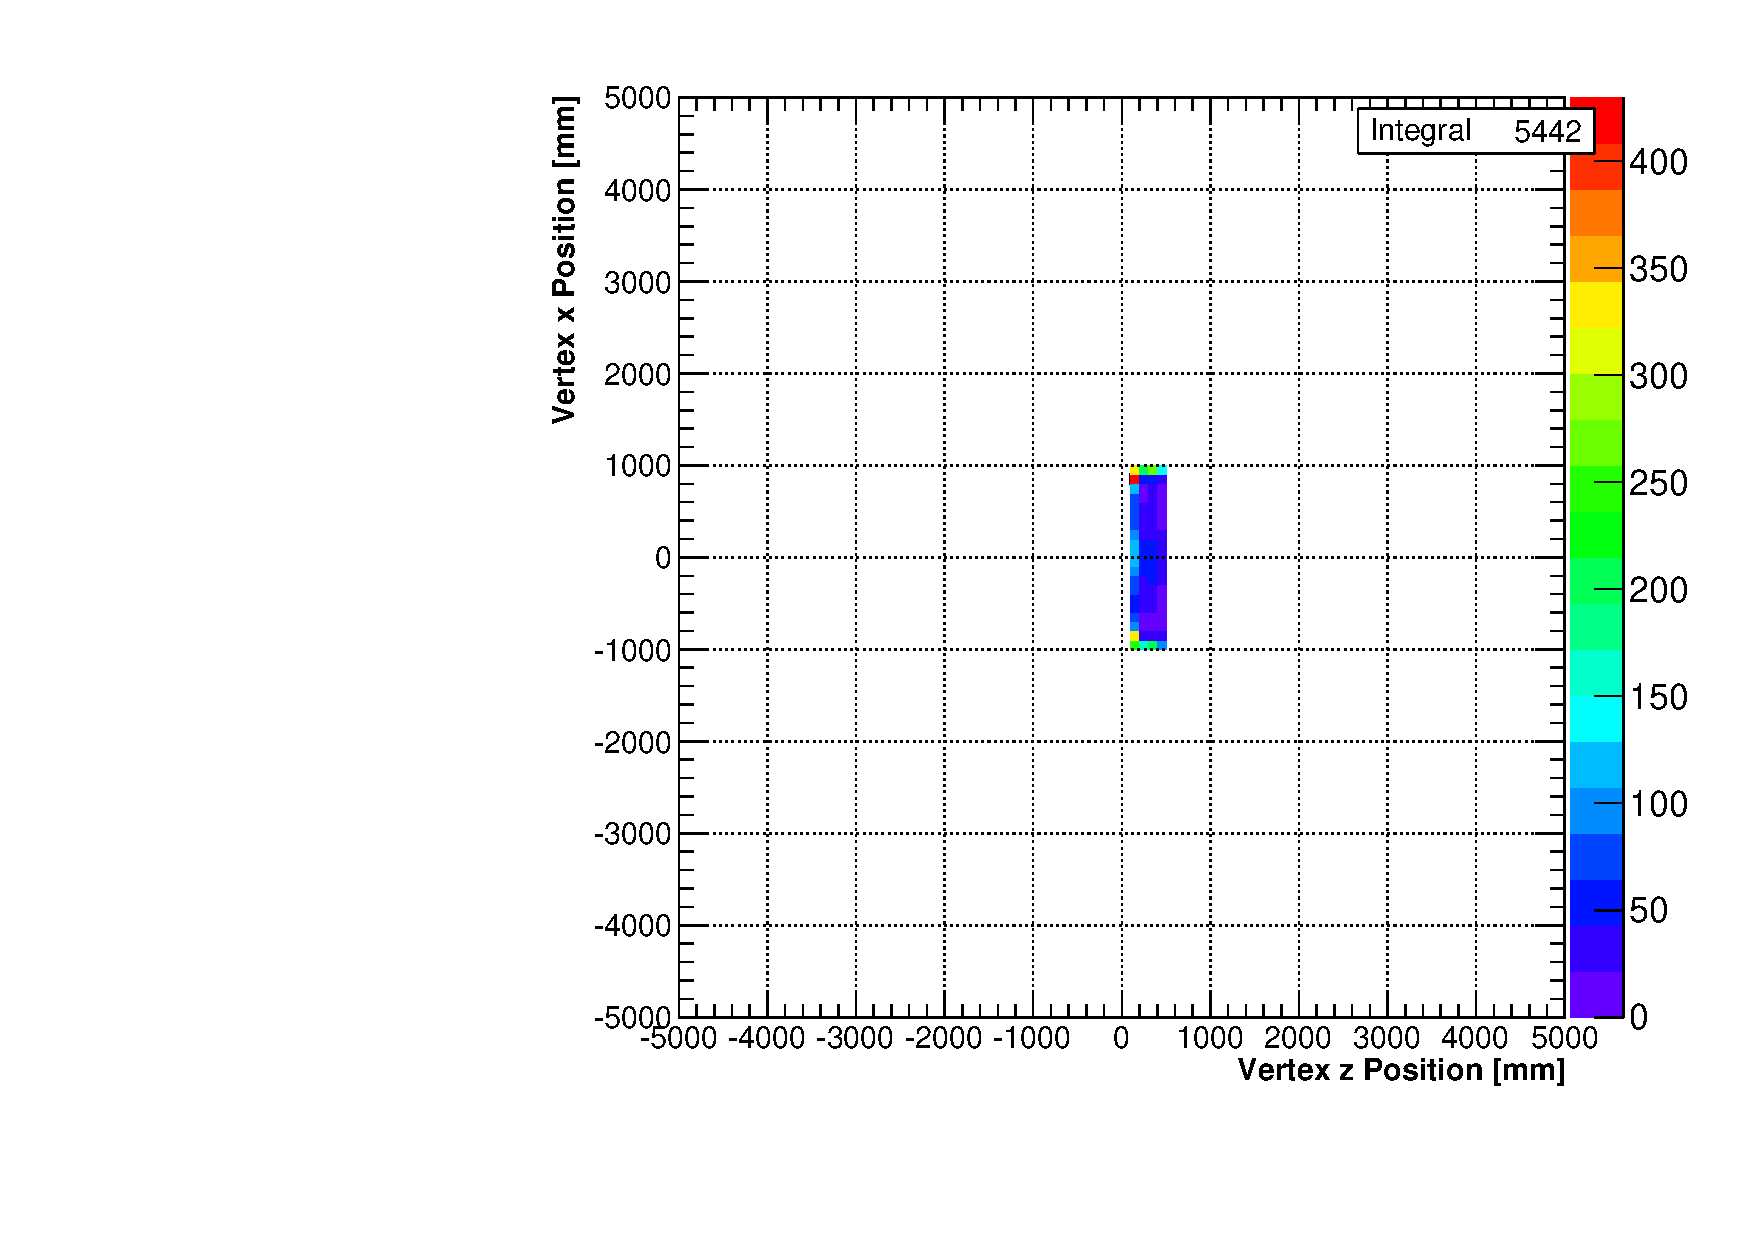
\includegraphics[width=0.48\textwidth]{T2K-TN-313/images/systematics/xz_oofv_reco.pdf} \\
  \caption[Reconstructed positions of the events selected for the
  estimation of the OOAFV error]{Same as
    Figure~\ref{fig:oofvcontrolsampletrue} for the reconstructed
    positions of the vertices.}
  \label{fig:oofvcontrolsamplereco}
\end{figure}

Next, the \Gls{FGD}1 \Gls{FV} events were used to reweight the
simulation for the events outside the fiducial volume
(\Gls{OOFV}). One can then assign the data~/~\Gls{MC} differences to
be due to a mass mis-modelling and assign uncertainties on each
component from these differences. This assumes that it is possible to
extrapolate the cross sections on elements that are in the support
structure from the \Gls{FGD}1 data. \cite{CallumRatios} shows that the
neutrino \Gls{CCQE} cross section implemented in the \Gls{NEUT}
generator is not necessarily reproducing well all the nuclear data
observed at \Gls{MINERVA}~\cite{MinervaRatios}.  However this study is
beyond the scope of this thesis, so it was assumed that the
uncertainties in ratio of the neutrino cross sections between
different targets are under control.

Since this is a geometrical effect, the contributions were categorised
according to their positions with respect to the \Gls{FGD}1. The
categories are bottom, top, back, left and right of the \Gls{FGD}1.

Note that this selection is extremely sensitive to the so-called
\gls{sand} interactions. These events happen outside the \Gls{ND}, in
the \gls{sand} surrounding it. The reason \gls{sand} events enter the
selection is because the vetoes do not work well for events next to
the edges of the \Gls{FGD}1: \gls{sand} muons come in between the
\Gls{P0DECal} and the \Gls{PD} and do not produce a visible signal in
the \Gls{TPC}1.

The results of this study and the mass uncertainties are given in
Table~\ref{tab:oofvmasserror}.  Note the great uncertainty of the $-y$
region: this is because there is a gap in the isolation between the
bottom left and right \Gls{BrECal} modules (which is used for
cabling). This is probably is not modelled well, therefore one can
expect some disagreements here.

\begin{table}[ht]
  \begin{adjustbox}{center}
    \begin{tabular}{cc}
      \toprule
      Region & Mass uncertainty \\ 
      \midrule
      $+x$     &  6.6506~\%  \\
      $-x$     &  6.0402~\%  \\
      $+y$     &  5.5572~\%  \\
      $-y$     & 38.2304~\%  \\
      $-z$     &  6.5380~\%  \\
      \bottomrule
    \end{tabular}
  \end{adjustbox}
  \caption[The FGD1 surroundings mass uncertainties]{The \Gls{FGD}1
    surroundings (\Gls{OOAFV}) mass uncertainties.}
  \label{tab:oofvmasserror}
\end{table}

\chapter{Photon reconstruction capabilities}
\label{app:rec}
Although there is no real motivation specific to the \Gls{NCg}
analysis to compute the resolutions, the use of the analysis could go
beyond a standard cross section analysis. Namely, computing
resolutions allows forward folding, when combined with the
efficiency. This would allow folding some more exotic models. In
Figure~\ref{fig:elecrecon}, the electrons~/~positrons reconstruction
capabilities are shown (after the \Gls{PID} cut) for one-dimensional
distributions (momentum and $\cos(\theta)$).

\begin{figure}[ht]
  \center
  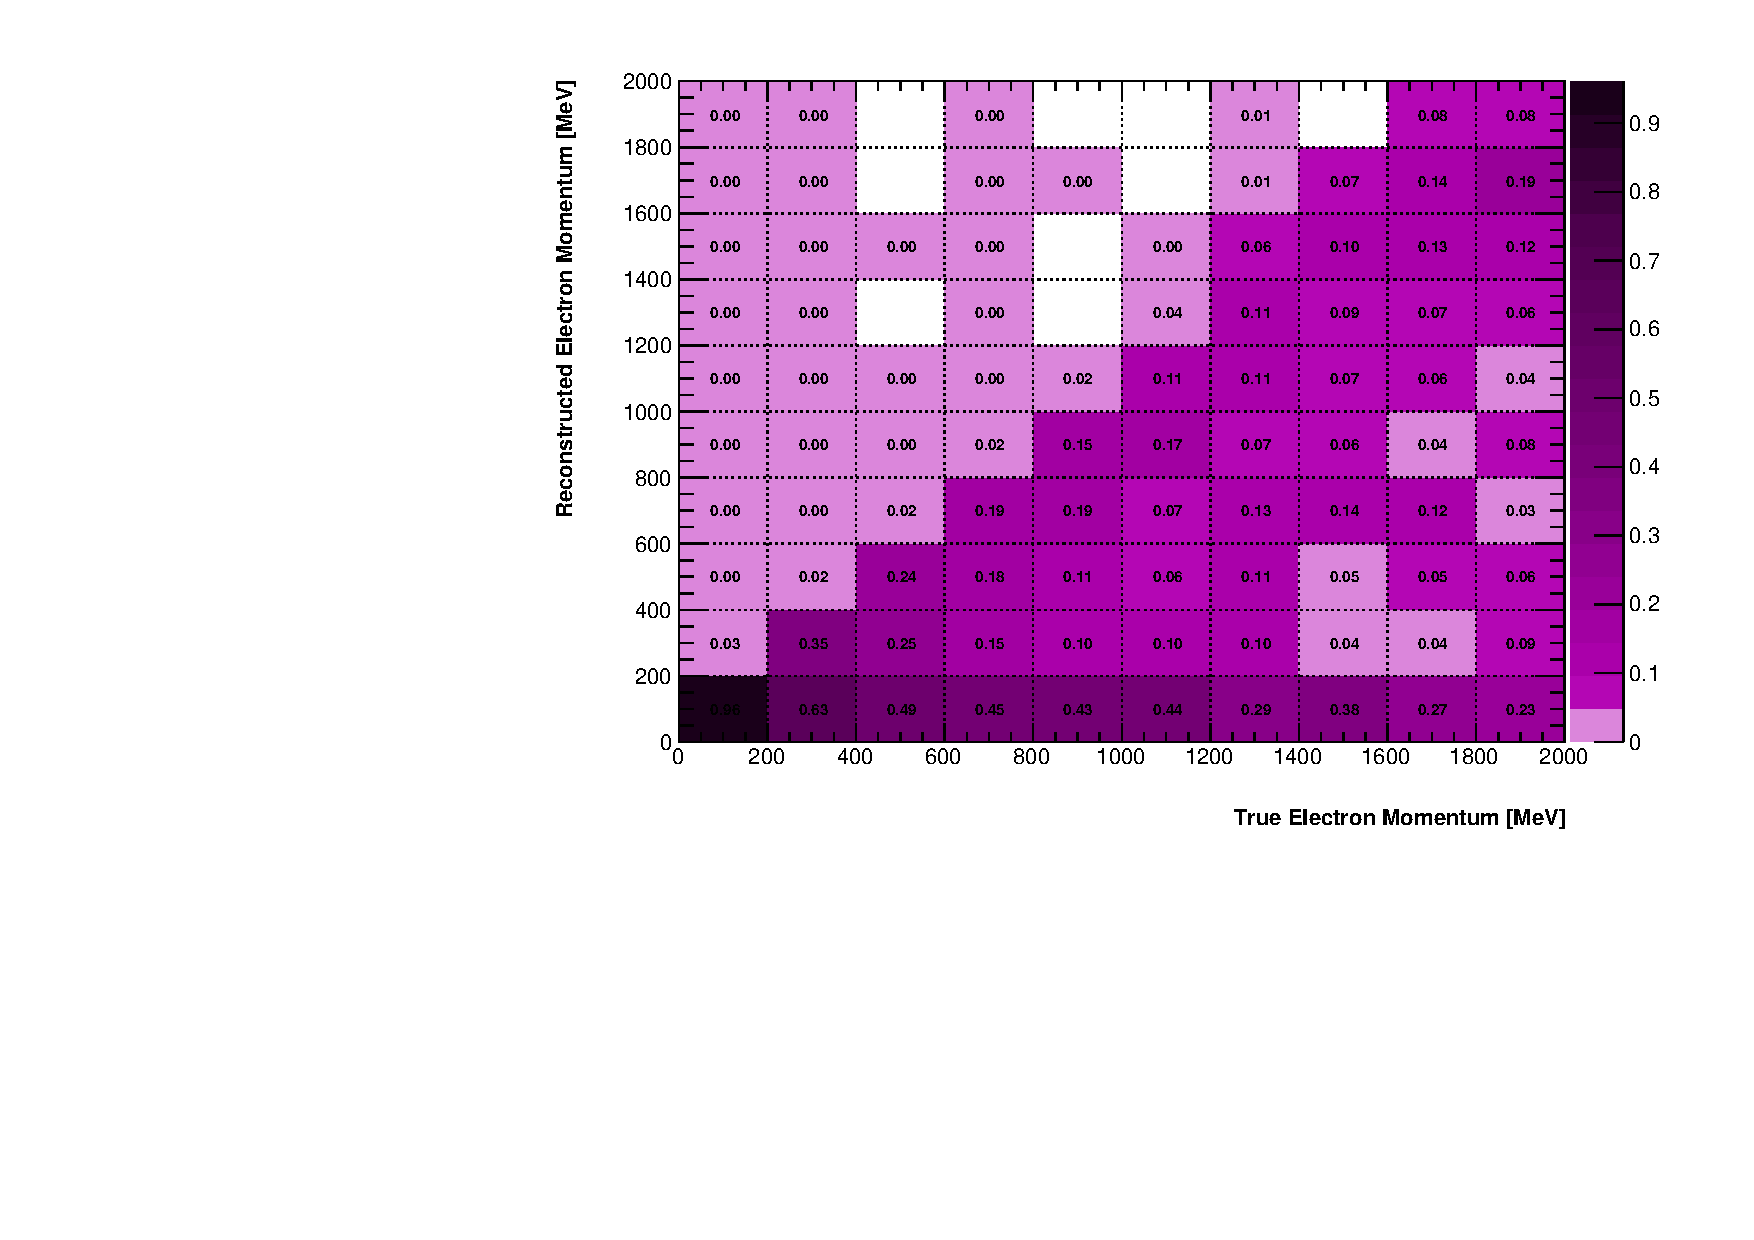
\includegraphics[width=0.8\textwidth]{T2K-TN-254/images/resol/0_MomResolutionElecton.pdf} \\
  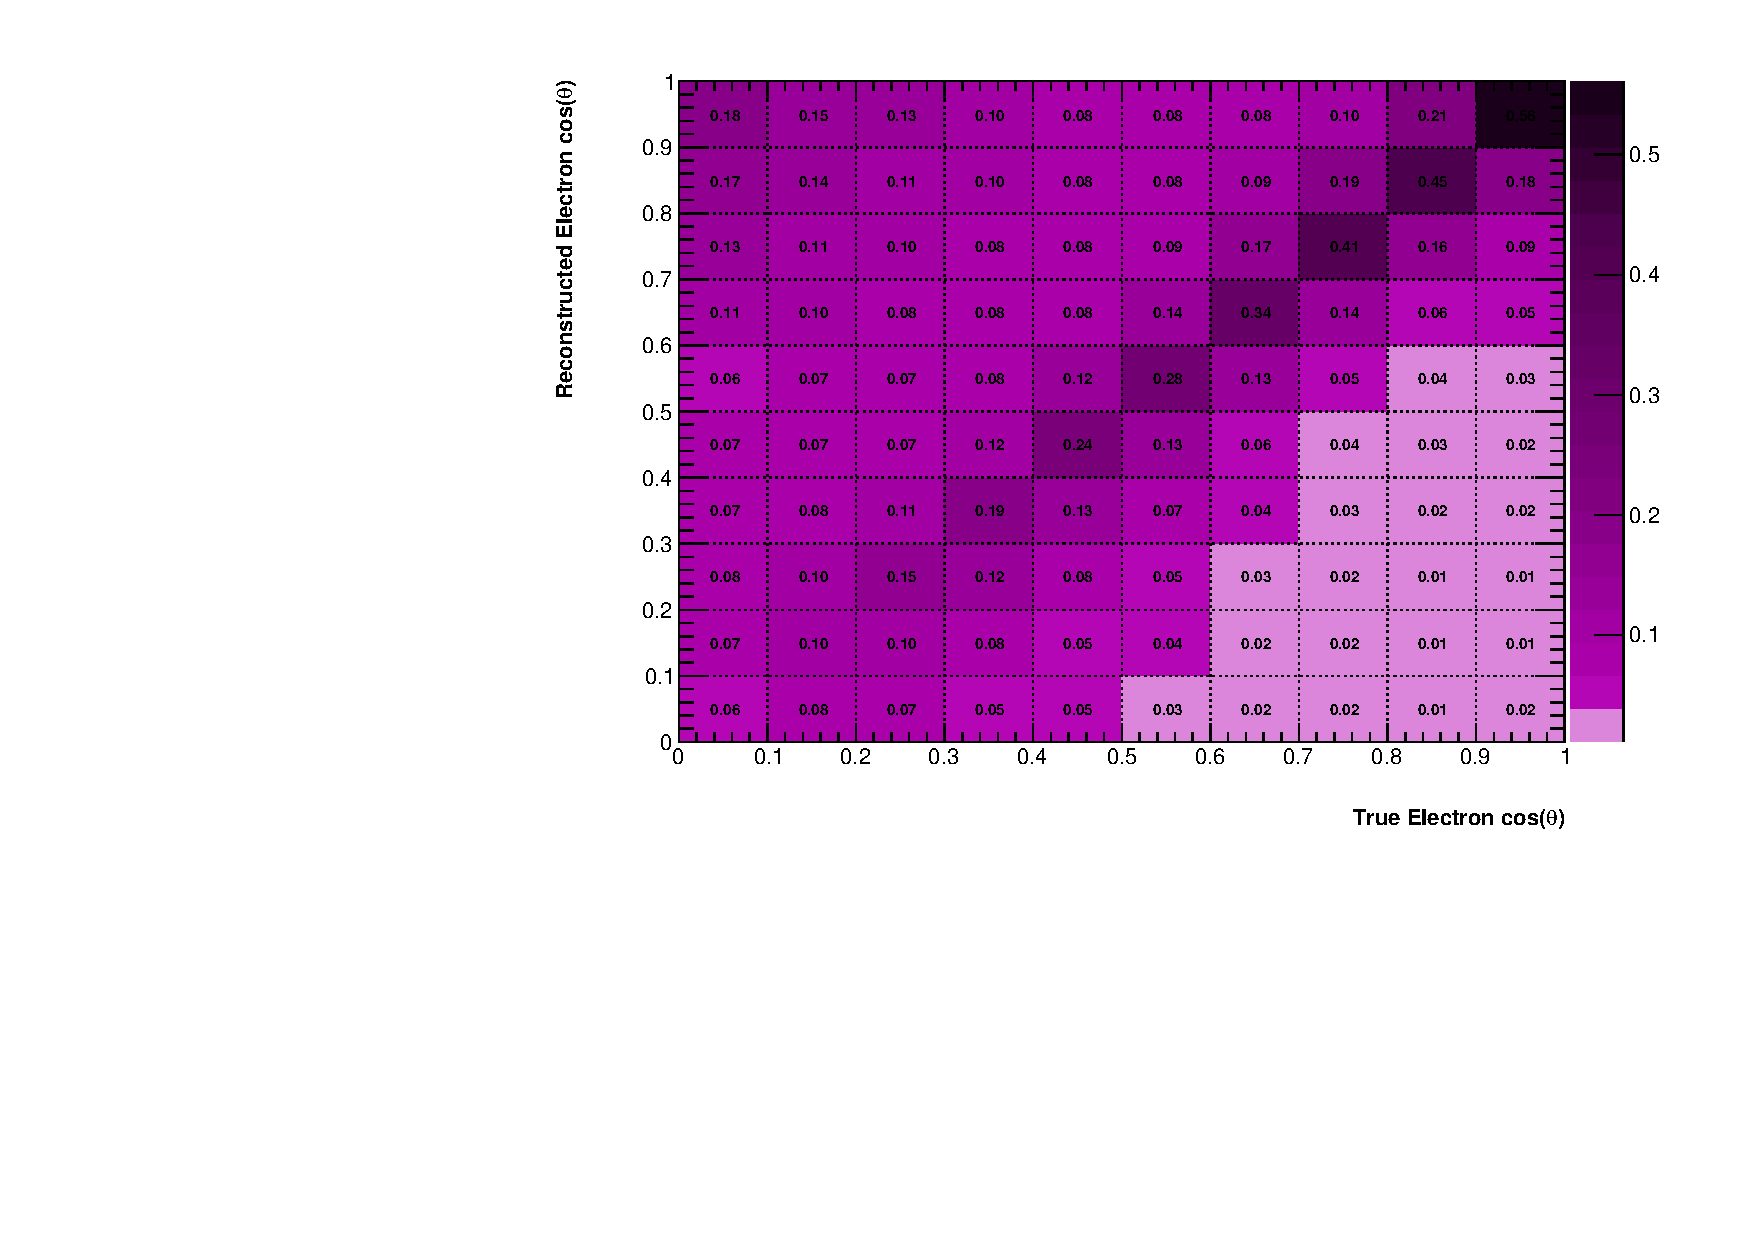
\includegraphics[width=0.8\textwidth]{T2K-TN-254/images/resol/1_CosResolutionElecton.pdf} 
  \caption[Electron~/~positron resolutions]{Electrons~/~positrons
    resolutions. \textbf{\textit{Top:}} Momentum
    resolution. \textbf{\textit{Bottom:}} Angular resolution.}
  \label{fig:elecrecon}
\end{figure}
Note the bias towards small reconstructed momentum which probably
comes from the Bremsstrahlung losses.

Next, the same quantities are computed for photons after the invariant
mass cut, in Figure~\ref{fig:photonrecon}.

\begin{figure}[ht]
  \center
  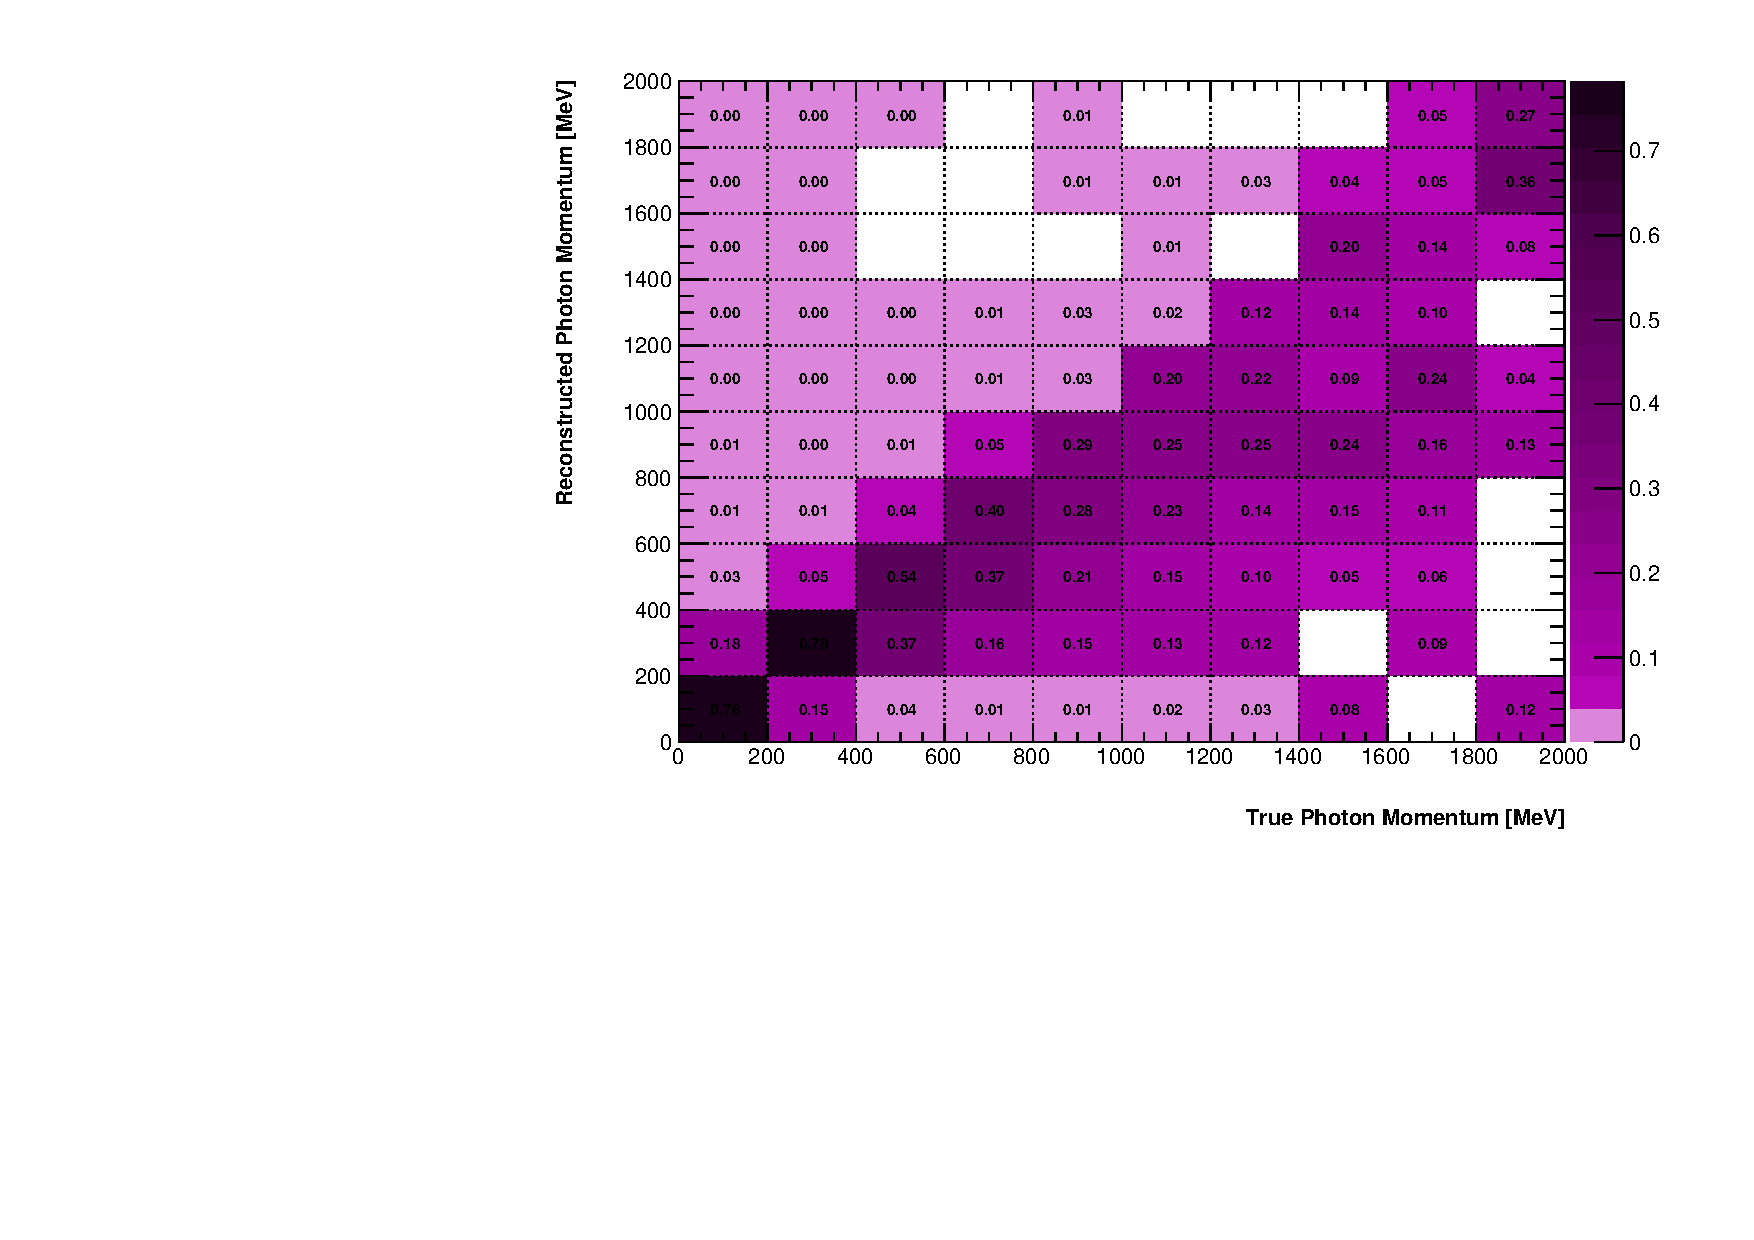
\includegraphics[width=0.8\textwidth]{T2K-TN-254/images/resol/0_MomResolutionGamma.pdf} 
  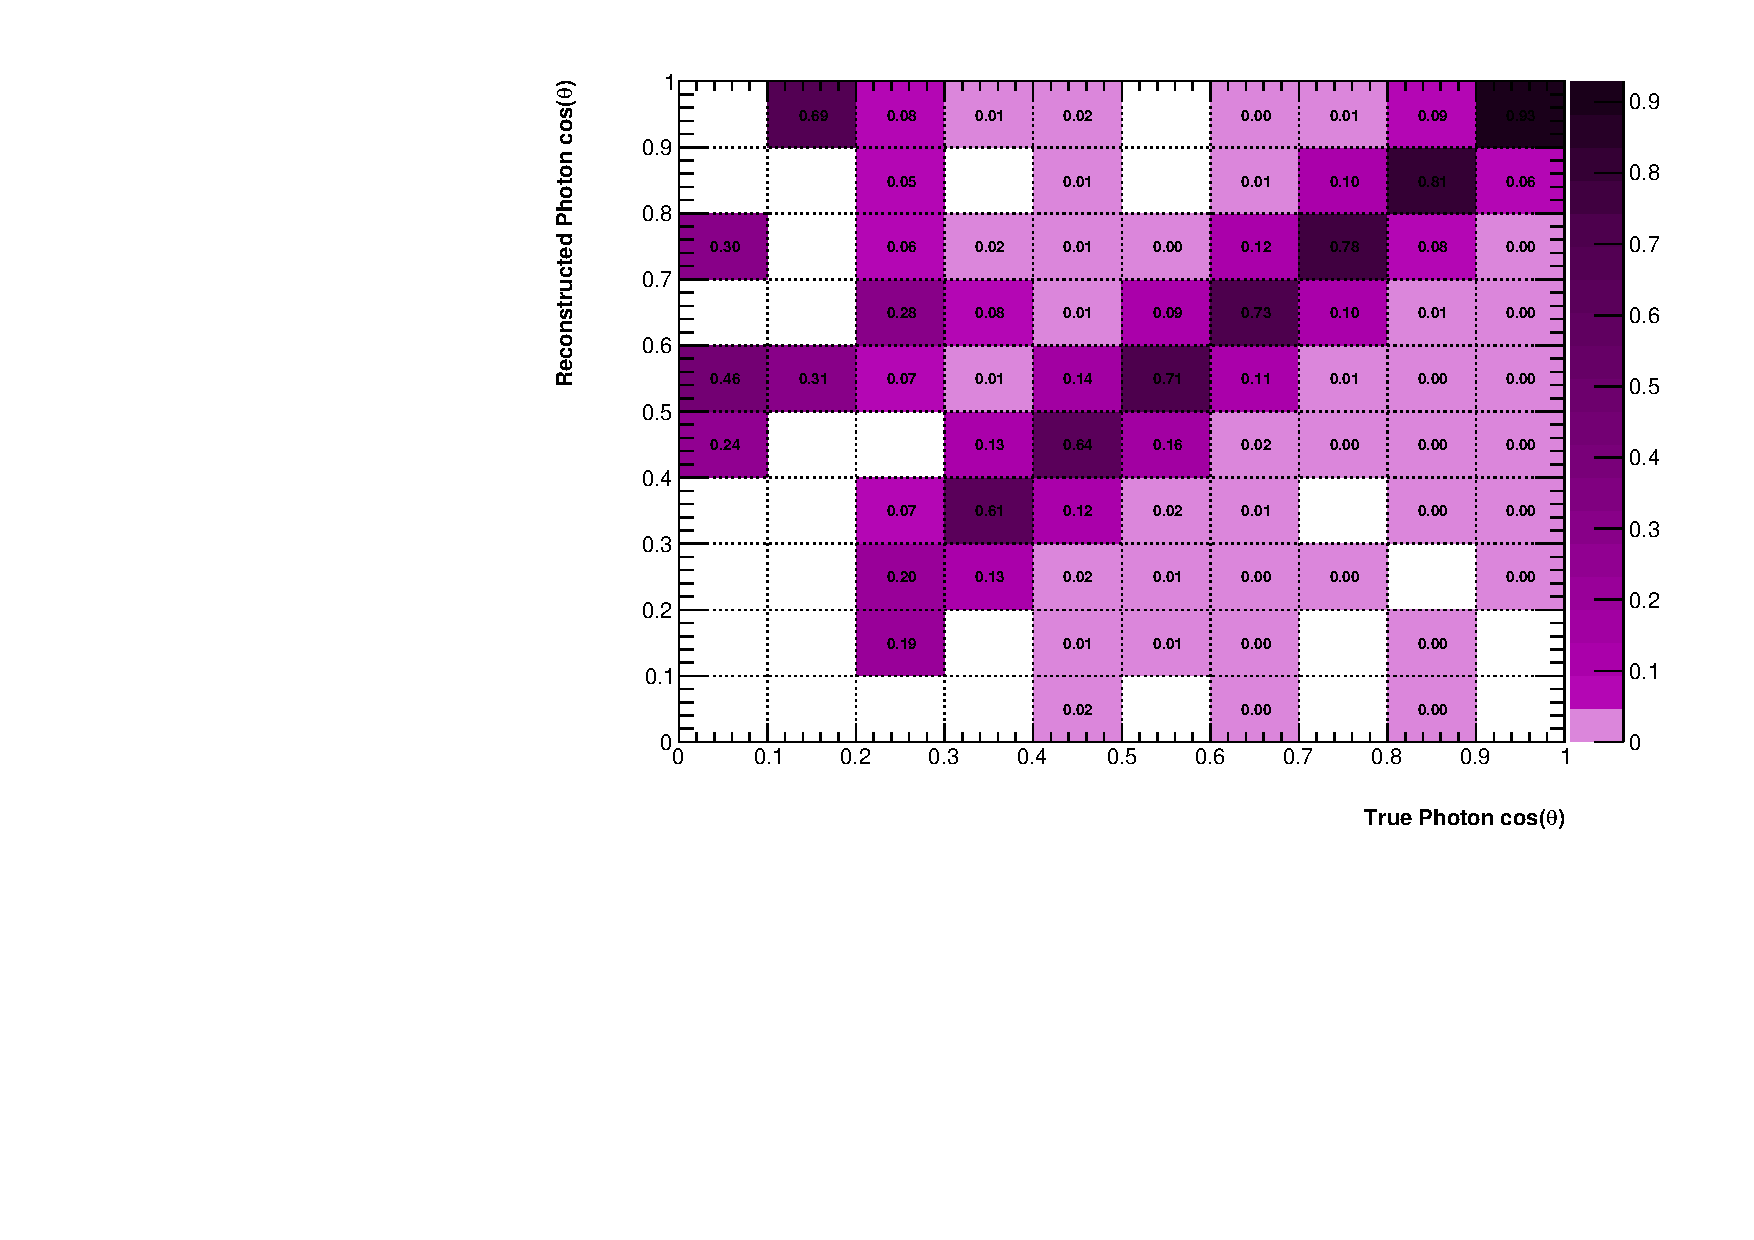
\includegraphics[width=0.8\textwidth]{T2K-TN-254/images/resol/2_CosResolutionGamma.pdf} 
  \caption[Photon resolutions]{Same as Figure~\ref{fig:elecrecon} for
    photons.}
  \label{fig:photonrecon}
\end{figure}

\clearpage
\newpage
\blankpage

\chapter{BANFF binning}
\label{app:binning}
In Chapter~\ref{chap:banff}, fits are performed over several samples
from the \Gls{ND}; these samples are binned in two dimensions
according to the lepton momentum ($p_l$, in MeV) and to the cosine of
the angle between the directions of the neutrino and the lepton
($\cos(\theta_l)$) . The binnings of the samples are given here in
details.

Firstly, the binning used in the fit for the construction of the
likelihood is:
\begin{itemize}
\item \Gls{FHC} \Gls{numu} \Gls{CC} $0\pi$ (\Gls{FGD}1 and 2):
  \begin{itemize}
  \item $p_\mu$: 14 bins, $\{0$, $300$, $400$, $500$, $600$, $700$, $800$, $900$, $1000$, $1250$, $1500$, $2000$, $3000$, $5000$, $30000\}$
  \item $\cos(\theta_\mu)$: 11 bins, $\{-1$, $0.6$, $0.7$, $0.8$, $0.85$, $0.9$, $0.92$, $0.94$, $0.96$, $0.98$, $0.99$, $1\}$
  \end{itemize}
\item \Gls{FHC} \Gls{numu} \Gls{CC} $1\pi$ (\Gls{FGD}1 and 2):
  \begin{itemize}
  \item $p_\mu$: 13 bins, $\{0$, $300$, $400$, $500$, $600$, $700$, $800$, $900$, $1000$, $1250$, $1500$, $2000$, $5000$, $30000\}$
  \item $\cos(\theta_\mu)$: 11 bins, $\{-1$, $0.6$, $0.7$, $0.8$, $0.85$, $0.9$, $0.92$, $0.94$, $0.96$, $0.98$, $0.99$, $1\}$
  \end{itemize} 
\item \Gls{FHC} \Gls{numu} \Gls{CC} other (\Gls{FGD}1 and 2):
  \begin{itemize}
  \item $p_\mu$: 14 bins, $\{0$, $300$, $400$, $500$, $600$, $700$, $800$, $900$, $1000$, $1250$, $1500$, $2000$, $3000$, $5000$, $30000\}$
  \item $\cos(\theta_\mu)$: 11 bins, $\{-1$, $0.6$, $0.7$, $0.8$, $0.85$, $0.90$, $0.92$, $0.94$, $0.96$, $0.98$, $0.99$, $1\}$
  \end{itemize}
\item \Gls{RHC} \Gls{anumu} \Gls{CC} $0\pi$ (\Gls{FGD}1 and 2):
  \begin{itemize}
  \item $p_\mu$: 8 bins, $\{0$, $300$, $500$, $700$, $900$, $1250$, $1500$, $2000$, $30000\}$
  \item $\cos(\theta_\mu)$: 10 bins, $\{-1$, $0.7$, $0.8$, $0.85$, $0.9$, $0.94$, $0.96$, $0.98$, $0.99$, $0.995$, $1\}$
  \end{itemize}
\item \Gls{RHC} \Gls{anumu} \Gls{CC} $1\pi$ (\Gls{FGD}1 and 2):
  \begin{itemize}
  \item $p_\mu$: 6 bins, $\{0$, $400$, $700$, $1000$, $1500$, $2500$, $30000\}$
  \item $\cos(\theta_\mu)$: 3 bins, $\{-1$, $0.8$, $0.9$, $1\}$
  \end{itemize} 
\item \Gls{RHC} \Gls{anumu} \Gls{CC} other (\Gls{FGD}1 and 2):
  \begin{itemize}
  \item $p_\mu$: 8 bins, $\{0$, $300$, $600$, $900$, $1200$, $1500$, $2000$, $4000$, $30000\}$
  \item $\cos(\theta_\mu)$: 4 bins, $\{-1$, $0.8$, $0.9$, $0.95$, $1\}$
  \end{itemize}
\item \Gls{RHC} \Gls{numu} \Gls{CC} $0\pi$ (\Gls{FGD}1 and 2):
  \begin{itemize}
  \item $p_\mu$: 6 bins, $\{0$, $350$, $700$, $1000$, $1500$, $2000$, $30000\}$
  \item $\cos(\theta_\mu)$: 7 bins, $\{-1$, $0.85$, $0.9$, $0.92$, $0.94$, $0.96$, $0.98$, $1\}$
  \end{itemize}
\item \Gls{RHC} \Gls{numu} \Gls{CC} $1\pi$ (\Gls{FGD}1 and 2):
  \begin{itemize}
  \item $p_\mu$: 8 bins, $\{0$, $350$, $500$, $650$, $800$, $1000$, $1250$, $2000$, $30000\}$
  \item $\cos(\theta_\mu)$: 4 bins, $\{-1$, $0.8$, $0.9$, $0.95$, $1\}$
  \end{itemize} 
\item \Gls{RHC} \Gls{numu} \Gls{CC} other (\Gls{FGD}1 and 2):
  \begin{itemize}
  \item $p_\mu$: 6 bins, $\{0$, $300$, $600$, $1000$, $2000$, $5000$, $30000\}$
  \item $\cos(\theta_\mu)$: 3 bins, $\{-1.$, $0.9$, $0.95$, $1\}$
  \end{itemize}
\item \Gls{FHC} \Gls{nue} \Gls{CC} inclusive (\Gls{FGD}1 and 2):
  \begin{itemize}
  \item $p_\mu$: 6 bins, $\{200$, $400$, $600$, $800$, $1000$, $1500$, $30000\}$
  \item $\cos(\theta_\mu)$: 3 bins, $\{-1$, $0.9$, $0.95$, $1\}$
  \end{itemize}
\item \Gls{FHC} photon (\Gls{FGD}1 and 2):
  \begin{itemize}
  \item $p_\mu$: 5 bins, $\{200$, $300$, $400$, $600$, $1000$, $30000\}$
  \item $\cos(\theta_\mu)$: 1 bin, $\{-1$, $1\}$
  \end{itemize}
\item \Gls{RHC} \Gls{anue} \Gls{CC} inclusive (\Gls{FGD}1 and 2):
  \begin{itemize}
  \item $p_\mu$: 3 bins, $\{200$, $500$, $1000$, $30000\}$
  \item $\cos(\theta_\mu)$: 2 bins, $\{-1$, $0.9$, $1\}$
  \end{itemize}
\item \Gls{RHC} \Gls{nue} \Gls{CC} inclusive (\Gls{FGD}1 and 2):
  \begin{itemize}
  \item $p_\mu$: 6 bins, $\{200$, $400$, $600$, $800$, $1000$, $2000$, $30000\}$
  \item $\cos(\theta_\mu)$: 2 bins, $\{-1$, $0.9$, $1\}$
  \end{itemize}
\item \Gls{RHC} photon (\Gls{FGD}1 and 2):
  \begin{itemize}
  \item $p_\mu$: 5 bins, $\{200$, $400$, $600$, $800$, $1000$, $30000\}$
  \item $\cos(\theta_\mu)$: 1 bin, $\{-1$, $1\}$.
  \end{itemize}
\end{itemize}
Therefore, the likelihood runs over $1438$ bins.
Next, the binning for the covariance is detailed:
\begin{itemize}
\item \Gls{FHC} \Gls{numu} \Gls{CC} $0\pi$ (\Gls{FGD}1 and 2):
  \begin{itemize}
  \item $p_\mu$: 6 bins, $\{0$, $1000$, $1250$, $2000$, $3000$, $5000$, $30000\}$
  \item $\cos(\theta_\mu)$: 7 bins, $\{-1$, $0.6$, $0.7$, $0.8$, $0.85$, $0.94$, $0.96$, $1\}$
  \end{itemize}
\item \Gls{FHC} \Gls{numu} \Gls{CC} $1\pi$ (\Gls{FGD}1 and 2):
  \begin{itemize}
  \item $p_\mu$: 5 bins, $\{0$, $300$, $1250$, $1500$, $5000$, $30000\}$
  \item $\cos(\theta_\mu)$: 8 bins, $\{-1$, $0.7$, $0.85$, $0.9$, $0.92$, $0.96$, $0.98$, $0.99$, $1\}$
  \end{itemize} 
\item \Gls{FHC} \Gls{numu} \Gls{CC} other (\Gls{FGD}1 and 2):
  \begin{itemize}
  \item $p_\mu$: 5 bins, $\{0$, $1500$, $2000$, $3000$, $5000$, $30000\}$
  \item $\cos(\theta_\mu)$: 8 bins, $\{-1$, $0.8$, $0.85$, $0.9$, $0.92$, $0.96$, $0.98$, $0.99$, $1\}$
  \end{itemize}  

\item \Gls{RHC} \Gls{anumu} \Gls{CC} $0\pi$ (\Gls{FGD}1 and 2):
  \begin{itemize}
  \item $p_\mu$: 4 bins, $\{0$, $900$, $1250$, $2000$, $30000\}$
  \item $\cos(\theta_\mu)$: 10 bins, $\{-1$, $0.7$, $0.8$, $0.85$, $0.9$, $0.94$, $0.96$, $0.98$, $0.99$, $0.995$, $1\}$
  \end{itemize}
\item \Gls{RHC} \Gls{anumu} \Gls{CC} $1\pi$ \Gls{FGD}1, \Gls{FGD}2 is
  the same as the likelihood binning:
  \begin{itemize}
  \item $p_\mu$: 4 bins, $\{0$, $400$, $1500$, $2500$, $30000\}$
  \item $\cos(\theta_\mu)$: 3 bins, $\{-1$, $0.8$, $0.9$, $1\}$
  \end{itemize} 
\item \Gls{RHC} \Gls{anumu} \Gls{CC} other (\Gls{FGD}1 and 2):
  \begin{itemize}
  \item $p_\mu$: 4 bins, $\{0$, $1500$, $2000$, $4000$, $30000\}$
  \item $\cos(\theta_\mu)$: 4 bins, $\{-1$, $0.8$, $0.9$, $0.95$, $1\}$
  \end{itemize}


  
\item \Gls{RHC} \Gls{numu} \Gls{CC} $0\pi$ (\Gls{FGD}1 and 2):
  \begin{itemize}
  \item $p_\mu$: 4 bins, $\{0$, $1000$, $1500$, $2000$, $30000\}$
  \item $\cos(\theta_\mu)$: 7 bins, $\{-1$, $0.85$, $0.9$, $0.92$, $0.94$, $0.96$, $0.98$, $1\}$
  \end{itemize}
\item \Gls{RHC} \Gls{numu} \Gls{CC} $1\pi$ \Gls{FGD}1, \Gls{FGD}2 is
  the same as the likelihood binning :
  \begin{itemize}
  \item $p_\mu$: 4 bins, $\{0$, $350$, $1250$, $2000$, $30000\}$
  \item $\cos(\theta_\mu)$: 4 bins, $\{-1$, $0.8$, $0.9$, $0.95$, $1\}$
  \end{itemize} 
\item \Gls{RHC} \Gls{numu} \Gls{CC} other (\Gls{FGD}1 and 2):
  \begin{itemize}
  \item $p_\mu$: 4 bins, $\{0$, $1000$, $2000$, $5000$, $30000\}$
  \item $\cos(\theta_\mu)$: 3 bins, $\{-1$, $0.9$, $0.95$, $1\}$
  \end{itemize}


  
\item \Gls{FHC} \Gls{nue} \Gls{CC} inclusive (\Gls{FGD}1 and 2):
  \begin{itemize}
  \item $p_\mu$: 6 bins, $\{200$, $400$, $600$, $800$, $1000$, $1500$, $30000\}$
  \item $\cos(\theta_\mu)$: 1 bin, $\{-1$, $1\}$
  \end{itemize}
\item \Gls{FHC} photon (\Gls{FGD}1 and 2):
  \begin{itemize}
  \item $p_\mu$: 5 bins, $\{200$, $300$, $400$, $600$, $1000$, $30000\}$
  \item $\cos(\theta_\mu)$: 1 bin, $\{-1$, $1\}$
  \end{itemize}
\item \Gls{RHC} \Gls{nue} \Gls{CC} inclusive (\Gls{FGD}1 and 2):
  \begin{itemize}
  \item $p_\mu$: 6 bins, $\{200$, $400$, $600$, $800$, $1000$, $2000$, $30000\}$
  \item $\cos(\theta_\mu)$: 1 bin, $\{-1$, $1\}$
  \end{itemize}
\item \Gls{RHC} \Gls{anue} \Gls{CC} inclusive (\Gls{FGD}1 and 2):
  \begin{itemize}
  \item $p_\mu$: 3 bins, $\{200$, $500$, $1000$, $30000\}$
  \item $\cos(\theta_\mu)$: 1 bin, $\{-1$, $1\}$
  \end{itemize}
\item \Gls{RHC} photon (\Gls{FGD}1 and 2):
  \begin{itemize}
  \item $p_\mu$: 5 bins, $\{200$, $400$, $600$, $800$, $1000$, $30000\}$
  \item $\cos(\theta_\mu)$: 1 bin, $\{-1$, $1\}$,
  \end{itemize}
\end{itemize}
all of which add up to $542$ bins (the size of the detector covariance matrix).


\chapter{BANFF postfit flux parameters}
\label{app:fluxparam}

In this appendix, the flux parameters are shown before and after fits
to the \Gls{Asimov} and the real data sets of the \Gls{ND}.

\begin{table}[ht!]
  \center
  \begin{tabular}{llll}
    \toprule
    Parameter & Prefit & \Gls{Asimov} fit & Data fit \\\midrule
    \Gls{ND} \Gls{FHC} \Gls{numu} 0& 1.0 $\pm$ 0.10 & 1.0 $\pm$ 0.06 & 0.97 $\pm$ 0.06 \\ 
    \Gls{ND} \Gls{FHC} \Gls{numu} 1& 1.0 $\pm$ 0.10 & 1.0 $\pm$ 0.07 & 0.96 $\pm$ 0.07 \\ 
    \Gls{ND} \Gls{FHC} \Gls{numu} 2& 1.0 $\pm$ 0.09 & 1.0 $\pm$ 0.06 & 0.96 $\pm$ 0.06 \\ 
    \Gls{ND} \Gls{FHC} \Gls{numu} 3& 1.0 $\pm$ 0.09 & 1.0 $\pm$ 0.05 & 0.96 $\pm$ 0.05 \\ 
    \Gls{ND} \Gls{FHC} \Gls{numu} 4& 1.0 $\pm$ 0.11 & 1.0 $\pm$ 0.06 & 0.95 $\pm$ 0.06 \\ 
    \Gls{ND} \Gls{FHC} \Gls{numu} 5& 1.0 $\pm$ 0.10 & 1.0 $\pm$ 0.05 & 0.96 $\pm$ 0.05 \\
    \Gls{ND} \Gls{FHC} \Gls{numu} 6& 1.0 $\pm$ 0.07 & 1.0 $\pm$ 0.04 & 0.97 $\pm$ 0.04 \\ 
    \Gls{ND} \Gls{FHC} \Gls{numu} 7& 1.0 $\pm$ 0.07 & 1.0 $\pm$ 0.04 & 0.96 $\pm$ 0.04 \\ 
    \Gls{ND} \Gls{FHC} \Gls{numu} 8& 1.0 $\pm$ 0.08 & 1.0 $\pm$ 0.05 & 0.93 $\pm$ 0.04 \\ 
    \Gls{ND} \Gls{FHC} \Gls{numu} 9& 1.0 $\pm$ 0.10 & 1.0 $\pm$ 0.05 & 0.90 $\pm$ 0.04 \\ 
    \Gls{ND} \Gls{FHC} \Gls{numu} 10& 1.0 $\pm$ 0.11 & 1.0 $\pm$ 0.05 & 0.91 $\pm$ 0.05 \\ 
    \Gls{ND} \Gls{FHC} \Gls{anumu} 0& 1.0 $\pm$ 0.10 & 1.0 $\pm$ 0.05 & 0.97 $\pm$ 0.04 \\ 
    \Gls{ND} \Gls{FHC} \Gls{anumu} 1& 1.0 $\pm$ 0.08 & 1.0 $\pm$ 0.05 & 0.91 $\pm$ 0.04 \\ 
    \Gls{ND} \Gls{FHC} \Gls{anumu} 2& 1.0 $\pm$ 0.08 & 1.0 $\pm$ 0.05 & 0.93 $\pm$ 0.04 \\ 
    \Gls{ND} \Gls{FHC} \Gls{anumu} 3& 1.0 $\pm$ 0.09 & 1.0 $\pm$ 0.05 & 0.93 $\pm$ 0.05 \\ 
    \Gls{ND} \Gls{FHC} \Gls{anumu} 4& 1.0 $\pm$ 0.09 & 1.0 $\pm$ 0.05 & 0.94 $\pm$ 0.04 \\ 
    \Gls{ND} \Gls{FHC} \Gls{nue} 0 & 1.0 $\pm$ 0.09 & 1.0 $\pm$ 0.06 & 0.97 $\pm$ 0.06 \\ 
    \Gls{ND} \Gls{FHC} \Gls{nue} 1 & 1.0 $\pm$ 0.09 & 1.0 $\pm$ 0.06 & 0.96 $\pm$ 0.06 \\ 
    \Gls{ND} \Gls{FHC} \Gls{nue} 2 & 1.0 $\pm$ 0.08 & 1.0 $\pm$ 0.06 & 0.98 $\pm$ 0.06 \\ 
    \Gls{ND} \Gls{FHC} \Gls{nue} 3 & 1.0 $\pm$ 0.08 & 1.0 $\pm$ 0.05 & 0.95 $\pm$ 0.05 \\ 
    \Gls{ND} \Gls{FHC} \Gls{nue} 4 & 1.0 $\pm$ 0.08 & 1.0 $\pm$ 0.05 & 0.96 $\pm$ 0.04 \\ 
    \Gls{ND} \Gls{FHC} \Gls{nue} 5 & 1.0 $\pm$ 0.08 & 1.0 $\pm$ 0.04 & 0.95 $\pm$ 0.04 \\ 
    \Gls{ND} \Gls{FHC} \Gls{nue} 6 & 1.0 $\pm$ 0.10 & 1.0 $\pm$ 0.06 & 0.98 $\pm$ 0.06 \\ 
    \Gls{ND} \Gls{FHC} \Gls{anue} 0& 1.0 $\pm$ 0.07 & 1.0 $\pm$ 0.05 & 0.98 $\pm$ 0.05 \\ 
    \Gls{ND} \Gls{FHC} \Gls{anue} 1& 1.0 $\pm$ 0.14 & 1.0 $\pm$ 0.11 & 1.13 $\pm$ 0.11 \\
    \bottomrule
  \end{tabular}
  \caption{\Gls{ND} \Gls{FHC} flux parameters values and uncertainties
    before and after an \Gls{Asimov} fit and a data fit.}
\end{table}
\begin{table}[ht!]
  \center
  \begin{tabular}{llll}
    \midrule
    Parameter & Prefit & \Gls{Asimov} fit & Data fit \\\midrule

    \Gls{ND} \Gls{RHC} \Gls{numu} 0& 1.0 $\pm$ 0.09 & 1.0 $\pm$ 0.04 & 0.95 $\pm$ 0.04 \\ 
    \Gls{ND} \Gls{RHC} \Gls{numu} 1& 1.0 $\pm$ 0.08 & 1.0 $\pm$ 0.04 & 0.93 $\pm$ 0.04 \\ 
    \Gls{ND} \Gls{RHC} \Gls{numu} 2& 1.0 $\pm$ 0.08 & 1.0 $\pm$ 0.04 & 0.93 $\pm$ 0.04 \\ 
    \Gls{ND} \Gls{RHC} \Gls{numu} 3& 1.0 $\pm$ 0.08 & 1.0 $\pm$ 0.04 & 0.96 $\pm$ 0.04 \\ 
    \Gls{ND} \Gls{RHC} \Gls{numu} 4& 1.0 $\pm$ 0.08 & 1.0 $\pm$ 0.03 & 0.81 $\pm$ 0.03 \\ 
    \Gls{ND} \Gls{RHC} \Gls{anumu} 0& 1.0 $\pm$ 0.11 & 1.0 $\pm$ 0.06 & 0.99 $\pm$ 0.06 \\ 
    \Gls{ND} \Gls{RHC} \Gls{anumu} 1& 1.0 $\pm$ 0.10 & 1.0 $\pm$ 0.07 & 0.97 $\pm$ 0.07 \\ 
    \Gls{ND} \Gls{RHC} \Gls{anumu} 2& 1.0 $\pm$ 0.09 & 1.0 $\pm$ 0.06 & 0.95 $\pm$ 0.06 \\ 
    \Gls{ND} \Gls{RHC} \Gls{anumu} 3& 1.0 $\pm$ 0.08 & 1.0 $\pm$ 0.05 & 0.95 $\pm$ 0.05 \\ 
    \Gls{ND} \Gls{RHC} \Gls{anumu} 4& 1.0 $\pm$ 0.11 & 1.0 $\pm$ 0.07 & 0.97 $\pm$ 0.07 \\ 
    \Gls{ND} \Gls{RHC} \Gls{anumu} 5& 1.0 $\pm$ 0.10 & 1.0 $\pm$ 0.07 & 0.96 $\pm$ 0.07 \\ 
    \Gls{ND} \Gls{RHC} \Gls{anumu} 6& 1.0 $\pm$ 0.07 & 1.0 $\pm$ 0.05 & 0.95 $\pm$ 0.05 \\ 
    \Gls{ND} \Gls{RHC} \Gls{anumu} 7& 1.0 $\pm$ 0.07 & 1.0 $\pm$ 0.05 & 0.96 $\pm$ 0.05 \\ 
    \Gls{ND} \Gls{RHC} \Gls{anumu} 8& 1.0 $\pm$ 0.09 & 1.0 $\pm$ 0.07 & 0.97 $\pm$ 0.07 \\ 
    \Gls{ND} \Gls{RHC} \Gls{anumu} 9& 1.0 $\pm$ 0.09 & 1.0 $\pm$ 0.06 & 0.97 $\pm$ 0.06 \\ 
    \Gls{ND} \Gls{RHC} \Gls{anumu} 10& 1.0 $\pm$ 0.13 & 1.0 $\pm$ 0.10 & 0.93 $\pm$ 0.10 \\ 
    \Gls{ND} \Gls{RHC} \Gls{nue} 0& 1.0 $\pm$ 0.07 & 1.0 $\pm$ 0.05 & 0.93 $\pm$ 0.05 \\ 
    \Gls{ND} \Gls{RHC} \Gls{nue} 1& 1.0 $\pm$ 0.09 & 1.0 $\pm$ 0.06 & 0.99 $\pm$ 0.06 \\ 
    \Gls{ND} \Gls{RHC} \Gls{anue} 0& 1.0 $\pm$ 0.10 & 1.0 $\pm$ 0.06 & 0.97 $\pm$ 0.06 \\ 
    \Gls{ND} \Gls{RHC} \Gls{anue} 1& 1.0 $\pm$ 0.09 & 1.0 $\pm$ 0.06 & 0.96 $\pm$ 0.06 \\ 
    \Gls{ND} \Gls{RHC} \Gls{anue} 2& 1.0 $\pm$ 0.09 & 1.0 $\pm$ 0.06 & 0.95 $\pm$ 0.06 \\ 
    \Gls{ND} \Gls{RHC} \Gls{anue} 3& 1.0 $\pm$ 0.08 & 1.0 $\pm$ 0.05 & 0.98 $\pm$ 0.05 \\ 
    \Gls{ND} \Gls{RHC} \Gls{anue} 4& 1.0 $\pm$ 0.08 & 1.0 $\pm$ 0.06 & 0.99 $\pm$ 0.06 \\ 
    \Gls{ND} \Gls{RHC} \Gls{anue} 5& 1.0 $\pm$ 0.09 & 1.0 $\pm$ 0.07 & 1.01 $\pm$ 0.07 \\ 
    \Gls{ND} \Gls{RHC} \Gls{anue} 6& 1.0 $\pm$ 0.16 & 1.0 $\pm$ 0.12 & 1.19 $\pm$ 0.12 \\ \bottomrule
  \end{tabular}
  \caption{\Gls{ND} \Gls{RHC} flux parameters values and uncertainties
    before and after an \Gls{Asimov} fit and a data fit.}
\end{table}
\begin{table}[ht!]
  \center
  \begin{tabular}{llll}
    \toprule
    Parameter & Prefit & \Gls{Asimov} fit & Data fit \\\midrule

    \Gls{SK} \Gls{FHC} \Gls{numu} 0& 1.0 $\pm$ 0.10 & 1.0 $\pm$ 0.07 & 0.97 $\pm$ 0.06 \\ 
    \Gls{SK} \Gls{FHC} \Gls{numu} 1& 1.0 $\pm$ 0.10 & 1.0 $\pm$ 0.07 & 0.97 $\pm$ 0.07 \\ 
    \Gls{SK} \Gls{FHC} \Gls{numu} 2& 1.0 $\pm$ 0.09 & 1.0 $\pm$ 0.06 & 0.96 $\pm$ 0.06 \\ 
    \Gls{SK} \Gls{FHC} \Gls{numu} 3& 1.0 $\pm$ 0.08 & 1.0 $\pm$ 0.05 & 0.95 $\pm$ 0.05 \\ 
    \Gls{SK} \Gls{FHC} \Gls{numu} 4& 1.0 $\pm$ 0.10 & 1.0 $\pm$ 0.06 & 0.95 $\pm$ 0.06 \\ 
    \Gls{SK} \Gls{FHC} \Gls{numu} 5& 1.0 $\pm$ 0.08 & 1.0 $\pm$ 0.05 & 0.96 $\pm$ 0.05 \\ 
    \Gls{SK} \Gls{FHC} \Gls{numu} 6& 1.0 $\pm$ 0.07 & 1.0 $\pm$ 0.04 & 0.97 $\pm$ 0.04 \\ 
    \Gls{SK} \Gls{FHC} \Gls{numu} 7& 1.0 $\pm$ 0.07 & 1.0 $\pm$ 0.05 & 0.97 $\pm$ 0.04 \\ 
    \Gls{SK} \Gls{FHC} \Gls{numu} 8& 1.0 $\pm$ 0.09 & 1.0 $\pm$ 0.05 & 0.93 $\pm$ 0.04 \\ 
    \Gls{SK} \Gls{FHC} \Gls{numu} 9& 1.0 $\pm$ 0.10 & 1.0 $\pm$ 0.04 & 0.88 $\pm$ 0.04 \\ 
    \Gls{SK} \Gls{FHC} \Gls{numu} 10& 1.0 $\pm$ 0.11 & 1.0 $\pm$ 0.06 & 0.91 $\pm$ 0.05 \\ 
    \Gls{SK} \Gls{FHC} \Gls{anumu} 0& 1.0 $\pm$ 0.10 & 1.0 $\pm$ 0.05 & 0.97 $\pm$ 0.05 \\ 
    \Gls{SK} \Gls{FHC} \Gls{anumu} 1& 1.0 $\pm$ 0.08 & 1.0 $\pm$ 0.05 & 0.94 $\pm$ 0.04 \\ 
    \Gls{SK} \Gls{FHC} \Gls{anumu} 2& 1.0 $\pm$ 0.08 & 1.0 $\pm$ 0.05 & 0.91 $\pm$ 0.05 \\ 
    \Gls{SK} \Gls{FHC} \Gls{anumu} 3& 1.0 $\pm$ 0.08 & 1.0 $\pm$ 0.05 & 0.91 $\pm$ 0.05 \\ 
    \Gls{SK} \Gls{FHC} \Gls{anumu} 4& 1.0 $\pm$ 0.09 & 1.0 $\pm$ 0.06 & 0.98 $\pm$ 0.06 \\ 
    \Gls{SK} \Gls{FHC} \Gls{nue} 0& 1.0 $\pm$ 0.09 & 1.0 $\pm$ 0.06 & 0.97 $\pm$ 0.06 \\ 
    \Gls{SK} \Gls{FHC} \Gls{nue} 1& 1.0 $\pm$ 0.09 & 1.0 $\pm$ 0.06 & 0.96 $\pm$ 0.06 \\ 
    \Gls{SK} \Gls{FHC} \Gls{nue} 2& 1.0 $\pm$ 0.08 & 1.0 $\pm$ 0.05 & 0.96 $\pm$ 0.05 \\ 
    \Gls{SK} \Gls{FHC} \Gls{nue} 3& 1.0 $\pm$ 0.08 & 1.0 $\pm$ 0.05 & 0.95 $\pm$ 0.04 \\ 
    \Gls{SK} \Gls{FHC} \Gls{nue} 4& 1.0 $\pm$ 0.08 & 1.0 $\pm$ 0.04 & 0.96 $\pm$ 0.04 \\ 
    \Gls{SK} \Gls{FHC} \Gls{nue} 5& 1.0 $\pm$ 0.08 & 1.0 $\pm$ 0.05 & 0.94 $\pm$ 0.04 \\ 
    \Gls{SK} \Gls{FHC} \Gls{nue} 6& 1.0 $\pm$ 0.09 & 1.0 $\pm$ 0.06 & 1.00 $\pm$ 0.06 \\ 
    \Gls{SK} \Gls{FHC} \Gls{anue} 0& 1.0 $\pm$ 0.07 & 1.0 $\pm$ 0.06 & 0.98 $\pm$ 0.05 \\ 
    \Gls{SK} \Gls{FHC} \Gls{anue} 1& 1.0 $\pm$ 0.13 & 1.0 $\pm$ 0.10 & 1.11 $\pm$ 0.10 \\ \bottomrule
  \end{tabular}
  \caption{\Gls{SK} \Gls{FHC} flux parameters values and uncertainties
    before and after an \Gls{Asimov} fit and a data fit.}
\end{table}


\begin{table}[ht!]
  \center
  \begin{tabular}{llll}
    \toprule
    Parameter & Prefit & \Gls{Asimov} fit & Data fit \\\midrule

    \Gls{SK} \Gls{RHC} \Gls{numu}  0& 1.0 $\pm$ 0.09 & 1.0 $\pm$ 0.04 & 0.96 $\pm$ 0.04 \\ 
    \Gls{SK} \Gls{RHC} \Gls{numu}  1& 1.0 $\pm$ 0.08 & 1.0 $\pm$ 0.05 & 0.94 $\pm$ 0.04 \\ 
    \Gls{SK} \Gls{RHC} \Gls{numu}  2& 1.0 $\pm$ 0.07 & 1.0 $\pm$ 0.04 & 0.93 $\pm$ 0.04 \\ 
    \Gls{SK} \Gls{RHC} \Gls{numu}  3& 1.0 $\pm$ 0.08 & 1.0 $\pm$ 0.05 & 0.92 $\pm$ 0.04 \\ 
    \Gls{SK} \Gls{RHC} \Gls{numu}  4& 1.0 $\pm$ 0.08 & 1.0 $\pm$ 0.04 & 0.88 $\pm$ 0.04 \\ 
    \Gls{SK} \Gls{RHC} \Gls{anumu} 0& 1.0 $\pm$ 0.11 & 1.0 $\pm$ 0.06 & 0.98 $\pm$ 0.06 \\ 
    \Gls{SK} \Gls{RHC} \Gls{anumu} 1& 1.0 $\pm$ 0.10 & 1.0 $\pm$ 0.07 & 0.97 $\pm$ 0.07 \\ 
    \Gls{SK} \Gls{RHC} \Gls{anumu} 2& 1.0 $\pm$ 0.09 & 1.0 $\pm$ 0.06 & 0.96 $\pm$ 0.06 \\ 
    \Gls{SK} \Gls{RHC} \Gls{anumu} 3& 1.0 $\pm$ 0.08 & 1.0 $\pm$ 0.05 & 0.95 $\pm$ 0.05 \\ 
    \Gls{SK} \Gls{RHC} \Gls{anumu} 4& 1.0 $\pm$ 0.10 & 1.0 $\pm$ 0.07 & 0.96 $\pm$ 0.07 \\ 
    \Gls{SK} \Gls{RHC} \Gls{anumu} 5& 1.0 $\pm$ 0.09 & 1.0 $\pm$ 0.06 & 0.95 $\pm$ 0.06 \\ 
    \Gls{SK} \Gls{RHC} \Gls{anumu} 6& 1.0 $\pm$ 0.07 & 1.0 $\pm$ 0.05 & 0.97 $\pm$ 0.05 \\ 
    \Gls{SK} \Gls{RHC} \Gls{anumu} 7& 1.0 $\pm$ 0.07 & 1.0 $\pm$ 0.05 & 0.97 $\pm$ 0.05 \\ 
    \Gls{SK} \Gls{RHC} \Gls{anumu} 8& 1.0 $\pm$ 0.09 & 1.0 $\pm$ 0.07 & 0.94 $\pm$ 0.07 \\ 
    \Gls{SK} \Gls{RHC} \Gls{anumu} 9& 1.0 $\pm$ 0.08 & 1.0 $\pm$ 0.06 & 0.91 $\pm$ 0.06 \\ 
    \Gls{SK} \Gls{RHC} \Gls{anumu} 10& 1.0 $\pm$ 0.11 & 1.0 $\pm$ 0.09 & 0.95 $\pm$ 0.09 \\ 
    \Gls{SK} \Gls{RHC} \Gls{nue}  0& 1.0 $\pm$ 0.07 & 1.0 $\pm$ 0.05 & 0.95 $\pm$ 0.05 \\ 
    \Gls{SK} \Gls{RHC} \Gls{nue}  1& 1.0 $\pm$ 0.08 & 1.0 $\pm$ 0.06 & 0.98 $\pm$ 0.06 \\ 
    \Gls{SK} \Gls{RHC} \Gls{anue} 0& 1.0 $\pm$ 0.10 & 1.0 $\pm$ 0.06 & 0.97 $\pm$ 0.06 \\ 
    \Gls{SK} \Gls{RHC} \Gls{anue} 1& 1.0 $\pm$ 0.09 & 1.0 $\pm$ 0.06 & 0.97 $\pm$ 0.05 \\ 
    \Gls{SK} \Gls{RHC} \Gls{anue} 2& 1.0 $\pm$ 0.09 & 1.0 $\pm$ 0.06 & 0.95 $\pm$ 0.05 \\ 
    \Gls{SK} \Gls{RHC} \Gls{anue} 3& 1.0 $\pm$ 0.08 & 1.0 $\pm$ 0.05 & 0.97 $\pm$ 0.05 \\ 
    \Gls{SK} \Gls{RHC} \Gls{anue} 4& 1.0 $\pm$ 0.08 & 1.0 $\pm$ 0.05 & 0.98 $\pm$ 0.05 \\ 
    \Gls{SK} \Gls{RHC} \Gls{anue} 5& 1.0 $\pm$ 0.09 & 1.0 $\pm$ 0.06 & 0.99 $\pm$ 0.06 \\ 
    \Gls{SK} \Gls{RHC} \Gls{anue} 6& 1.0 $\pm$ 0.15 & 1.0 $\pm$ 0.12 & 1.17 $\pm$ 0.12 \\
    \bottomrule
  \end{tabular}
  \caption{\Gls{SK} \Gls{RHC} flux parameters values and uncertainties
    before and after an \Gls{Asimov} fit and a data fit.}
\end{table}




%%% Local Variables:
%%% mode: latex
%%% TeX-master: "Thesis"
%%% End:
